\documentclass[10pt,a4paper]{article}
\usepackage[utf8]{inputenc}
\usepackage[T1]{fontenc}
\usepackage[spanish]{babel}
\usepackage{geometry}
\usepackage{hyperref}
\usepackage{setspace}
\usepackage{amsmath,amssymb}
\usepackage{graphicx}
\usepackage{xcolor}
\usepackage{titlesec}
\usepackage{parskip}
\usepackage{enumitem}
\usepackage{caption}
\usepackage{float}
\usepackage{array}
\usepackage{tabularx}
\usepackage{longtable}
\usepackage{pdflscape}
\usepackage{adjustbox}
\usepackage{forest}
\usepackage{listings}
\geometry{top=1.6cm, left=1.5cm, right=1.5cm, bottom=2cm}

\setstretch{1.05}
\setlength{\parindent}{0pt}
\setlength{\parskip}{4pt}
\setlength{\tabcolsep}{4pt}
\setlength{\emergencystretch}{3em}
\captionsetup{font=small, labelfont=bf}

\addto\captionsspanish{%
  \renewcommand{\figurename}{Figura}
  \renewcommand{\tablename}{Tabla}%
}

\titleformat{\section}{\normalfont\Large\bfseries}{\thesection}{1em}{}
\titleformat{\subsection}{\normalfont\large\bfseries}{\thesubsection}{1em}{}
\titleformat{\subsubsection}{\normalfont\normalsize\bfseries}{\thesubsubsection}{1em}{}

\hypersetup{colorlinks=true, linkcolor=blue, urlcolor=blue, citecolor=black}

\renewcommand{\arraystretch}{1.25}

% ---------- Macros de notación ----------
\newcommand{\nt}[1]{\ensuremath{\langle}\textit{#1}\ensuremath{\rangle}}   % no terminal
\newcommand{\tm}[1]{\texttt{#1}}                                          % terminal
\newcommand{\pend}[1]{\textcolor{red}{\textbf{[Pendiente: #1]}}}          % por completar
\newcommand{\pp}{\textcolor{red}{\scriptsize\textbf{pend.}}}
\newcolumntype{L}[1]{>{\raggedright\arraybackslash}p{#1}}
\newcolumntype{C}[1]{>{\centering\arraybackslash}p{#1}}
% ancho de columna como fracción exacta del ancho de línea (evita desbordes)
\newcommand{\cw}[1]{\dimexpr #1\linewidth-2\tabcolsep-\arrayrulewidth-0.4pt\relax}

% ---------- Listados de código ----------
\lstset{
  basicstyle=\ttfamily\footnotesize,
  frame=single,
  breaklines=true,
  columns=fullflexible,
  keepspaces=true,
  showstringspaces=false,
  extendedchars=true,
  literate={á}{{\'a}}1 {é}{{\'e}}1 {í}{{\'i}}1 {ó}{{\'o}}1 {ú}{{\'u}}1
           {ñ}{{\~n}}1 {Á}{{\'A}}1 {É}{{\'E}}1 {Í}{{\'I}}1 {Ó}{{\'O}}1 {Ú}{{\'U}}1
           {°}{{\textdegree}}1 {→}{{$\rightarrow$}}1
}

% ---------- Estilos para los árboles ----------
\forestset{
  nt/.style={draw, rounded corners=2pt, inner sep=2pt},
  term/.style={draw, font=\ttfamily, inner sep=2pt, fill=gray!12},
  lex/.style={font=\ttfamily\small, text=black, edge={dashed, blue}},
  ast/.style={draw, rounded corners=2pt, inner sep=3pt},
  astleaf/.style={draw, font=\ttfamily\small, inner sep=3pt, fill=gray!12},
}

\begin{document}
\shorthandoff{"<>}

% ============================================================
% PORTADA
% ============================================================
\begin{titlepage}
\centering

\IfFileExists{figuras/uct_fac.png}{
\includegraphics[width=3cm]{figuras/uct_fac.png}\\[1cm]}{\vspace*{3cm}}

{\Large \textbf{INFO1148}}\\[0.2cm]
{\large Teoría de la Computación}\\[2cm]

\rule{0.85\textwidth}{0.6pt}\\[0.4cm]
{\Huge \textbf{Proyecto}}\\[0.3cm]
{\Large Diseño e implementación de un analizador sintáctico}\\
{\Large ARMLANG: lenguaje de control para un brazo robótico clasificador}\\[0.4cm]
\rule{0.85\textwidth}{0.6pt}\\[2cm]

\begin{tabular}{@{}ll@{}}
\textbf{Integrante 1:} & Vicente Álvarez \\[0.15cm]
\textbf{Correo institucional:} & vicente.alvarez2023@alu.uct.cl \\[0.5cm]
\textbf{Integrante 2:} & Joaquín Cantero \\[0.15cm]
\textbf{Correo institucional:} & jcantero2023@alu.uct.cl \\[0.5cm]
\textbf{Integrante 3 (jefe):} & Juan Sepúlveda \\[0.15cm]
\textbf{Correo institucional:} & juan.sepulveda2023@alu.uct.cl \\
\end{tabular}

\vfill

\begin{tabular}{@{}ll@{}}
\textbf{Carrera:} & Ingeniería Civil en Informática \\[0.3cm]
\textbf{Docente:} & Marcos Lévano \\[0.3cm]
\textbf{Fecha de entrega:} & 1 de noviembre, 2026 \\
\end{tabular}

\vspace{1cm}
\end{titlepage}

\tableofcontents
\newpage

% ============================================================
% 1. INTRODUCCIÓN Y DOMINIO
% ============================================================
\section{Introducción y dominio seleccionado}
\label{sec:intro}

Este proyecto consiste en diseñar un pequeño lenguaje de dominio específico (DSL)
y construir un analizador sintáctico que reconozca los programas escritos en él,
avise cuando hay errores y entregue una representación estructurada de lo que
leyó. Todo el diseño se apoya en una gramática libre de contexto (GLC), en los
conjuntos FIRST y FOLLOW y en una tabla predictiva LL(1).

El dominio que elegimos es el \textbf{control de un brazo robótico clasificador}.
El brazo está junto a una cinta transportadora, toma pelotitas de distintos
materiales con una pinza, mide su peso y las deja en uno de tres contenedores
(aluminio, hierro y un material más pesado). Al lenguaje lo llamamos
\textbf{ARMLANG}. Escogimos este dominio porque la tarea tiene una estructura
clara que se traduce bien a una gramática: hay reglas que reaccionan a un sensor,
acciones con parámetros y una decisión con varias ramas (la clasificación por
peso), que es nuestra extensión creativa.

\subsection{La gramática responde a lo que el brazo necesita}

Queremos dejar claro desde el comienzo que la gramática no se diseñó en
abstracto. Primero escribimos qué necesitamos poder pedirle al brazo y recién
después buscamos qué construcciones de la gramática lo permiten. Cada producción
del lenguaje existe porque cubre alguno de estos requisitos de control.

\begin{table}[H]
\centering\small
\begin{tabularx}{\linewidth}{|C{0.9cm}|X|X|}
\hline
\textbf{N.°} & \textbf{Qué necesita el brazo} & \textbf{Construcción de la gramática que lo cubre} \\
\hline
R1 & Reaccionar al valor de un sensor (booleano o numérico). & Regla \tm{WHEN condicion THEN bloque} y comparación \tm{ID OP\_REL valor}. \\
\hline
R2 & Tener varias reglas independientes en un mismo programa. & \nt{programa} y \nt{reglas}. \\
\hline
R3 & Combinar varios sensores en una sola condición, con prioridad y agrupación. & \tm{OR}, \tm{AND}, \tm{NOT} y paréntesis. \\
\hline
R4 & Girar la base y subir o bajar el brazo a un ángulo dado. & \tm{MOVER articulacion NUM}. \\
\hline
R5 & Abrir y cerrar la pinza. & \tm{ABRIR PINZA} y \tm{CERRAR PINZA}. \\
\hline
R6 & Ejecutar varias acciones en un orden determinado. & \nt{bloque} con una lista de \nt{sentencias}. \\
\hline
R7 & Decidir según el peso medido a qué contenedor ir. & Decisión \tm{IF}--\tm{ELSE IF}--\tm{ELSE}. \\
\hline
R8 & Rechazar órdenes sin sentido físico por su estructura (por ejemplo, mover la pinza como si fuera una articulación). & \nt{articulacion} solo admite \tm{BASE} y \tm{BRAZO}. \\
\hline
R9 & Poder sumar sensores, partes o acciones, e incluso usar el lenguaje en otro brazo, sin rehacer la gramática. & Los sensores son \tm{ID}; las partes y acciones nuevas entran como un terminal y una producción (sección~\ref{sec:extensible}). \\
\hline
\end{tabularx}
\caption{Requisitos de control del brazo y la parte de la gramática que los cubre.}
\label{tab:requisitos_brazo}
\end{table}

\subsection{Organización del informe y cobertura de la rúbrica}

El informe sigue el orden que sugiere el enunciado. La Tabla~\ref{tab:rubrica} indica en qué
sección se encuentra la evidencia de cada criterio de la rúbrica. Los conjuntos FIRST, FOLLOW y de predicción, y la tabla LL(1), se calcularon aplicando las reglas
de la sección~\ref{sec:firstfollow} y se verificaron con un script auxiliar
(\tm{verificador\_ll1.py}), que solo sirve para contrastar los resultados y no reemplaza al parser del proyecto. El uso de IA se declara en el \hyperlink{anexoD}{Anexo D}”

\begin{table}[H]
\centering\small
\begin{tabularx}{\linewidth}{|L{0.30\linewidth}|C{0.9cm}|X|}
\hline
\textbf{Criterio de la rúbrica} & \textbf{Pts.} & \textbf{Dónde se encuentra} \\
\hline
1. Lenguaje y dominio & 10 & Secciones~\ref{sec:intro} y~\ref{sec:lenguaje}: propósito, alfabeto formal (sección~\ref{sec:alfabeto}), tokens (Tabla~\ref{tab:tokens}), ejemplos válidos (sección~\ref{sec:ej_validos}) e inválidos (Tabla~\ref{tab:invalidas}). \\
\hline
2. Gramática libre de contexto & 15 & Sección~\ref{sec:gramatica}: símbolo inicial, terminales, no terminales y las 33 producciones (sección~\ref{sec:gramatica_completa}); definición formal en el \hyperlink{anexoC}{Anexo C}. \\
\hline
3. Análisis, FIRST y FOLLOW & 20 & Sección~\ref{sec:analisis}: recursión (\ref{sec:recursion}), factorización (\ref{sec:factorizacion}) y ambigüedad (\ref{sec:ambiguedad}). Sección~\ref{sec:firstfollow}: FIRST (Tabla~\ref{tab:first}), FOLLOW (Tabla~\ref{tab:follow}) y predicción (Tabla~\ref{tab:pred}), todos justificados. \\
\hline
4. Tabla LL(1) & 10 & Sección~\ref{sec:tabla}: tabla completa (Tabla~\ref{tab:matriz}), ausencia de conflictos (sección~\ref{sec:conflictos}) y traza de ejemplo (Tabla~\ref{tab:traza}). \\
\hline
5. Implementación del parser & 20 & Sección~\ref{sec:parser}: descenso recursivo, una función por no terminal y correspondencia con la gramática (Tabla~\ref{tab:mapa}). \\
\hline
6. Árbol/AST y errores & 10 & Sección~\ref{sec:ast} (nodos en la Tabla~\ref{tab:ast}) y sección~\ref{sec:errores} (ejemplos en la Tabla~\ref{tab:ej_errores}). \\
\hline
7. Pruebas y extensión creativa & 10 & Extensión \tm{IF}--\tm{ELSE}: sección~\ref{sec:extension}. Pruebas (27 casos): sección~\ref{sec:pruebas}, Tablas~\ref{tab:validos}, \ref{tab:invalidos_casos} y~\ref{tab:limite}. \\
\hline
8. Informe y README & 5 & Todo el documento; \hyperlink{anexoA}{Anexo A} (repositorio y README) y \hyperlink{anexoB}{Anexo B} (demostración funcional). \\
\hline
\end{tabularx}
\caption{Cobertura de la rúbrica.}
\label{tab:rubrica}
\end{table}

% ============================================================
% 2. ESPECIFICACIÓN DEL LENGUAJE
% ============================================================
\section{Especificación del lenguaje}
\label{sec:lenguaje}

\subsection{Propósito del lenguaje}

ARMLANG permite escribir el programa de control de un brazo clasificador. Un
programa es una secuencia de \emph{reglas}, y cada regla dice ``cuando se cumpla
esta condición sobre los sensores, ejecuta este bloque de acciones''. Dentro del
bloque se pueden mover las articulaciones, abrir o cerrar la pinza y decidir con
\tm{IF}/\tm{ELSE} según el peso medido.

\subsection{Modelo físico del brazo}

El brazo tiene tres elementos móviles y dos sensores. El antebrazo va unido al
brazo mediante la articulación, pero no se mueve por sí solo, así que no entra al
lenguaje.

\begin{table}[H]
\centering\small
\begin{tabularx}{\linewidth}{|L{0.17\linewidth}|L{0.28\linewidth}|X|}
\hline
\textbf{Elemento} & \textbf{Función} & \textbf{Posiciones o valores relevantes} \\
\hline
\tm{BASE} & Gira el brazo completo sobre su eje. & 0° cinta; 60° contenedor de piezas livianas (aluminio); 120° piezas medias (hierro); 180° piezas pesadas. \\
\hline
\tm{BRAZO} & Articulación entre brazo y antebrazo: sube y baja. & 120° posición de reposo y de traslado; 30° posición de recoger y de soltar. \\
\hline
\tm{PINZA} & Agarra la pelotita. & Se abre (\tm{ABRIR}) y se cierra (\tm{CERRAR}). \\
\hline
\tm{pieza\_detectada} & Sensor de la cinta. & Booleano: hay o no una pieza lista para recoger. \\
\hline
\tm{peso} & Sensor de la pinza. & Numérico (gramos): solo mide cuando la pieza ya está agarrada. \\
\hline
\end{tabularx}
\caption{Elementos del brazo y sus posiciones.}
\label{tab:brazo}
\end{table}

El ciclo de trabajo del brazo, que es lo que describe un programa ARMLANG, es el siguiente:

\begin{table}[H]
\centering\small
\begin{tabularx}{\linewidth}{|C{1cm}|X|L{0.36\linewidth}|}
\hline
\textbf{Paso} & \textbf{Qué ocurre} & \textbf{Posición resultante} \\
\hline
0 & El brazo espera apuntando a la cinta. & base 0°, brazo 120° \\
\hline
1 & Baja a recoger la pieza. & brazo 30° \\
\hline
2 & Cierra la pinza (ahora el sensor \tm{peso} puede medir). & pinza cerrada \\
\hline
3 & Sube para moverse libre. & brazo 120° \\
\hline
4 & Gira al contenedor que corresponde según el peso. & base 60°, 120° o 180° \\
\hline
5 & Baja y suelta la pieza. & brazo 30°, pinza abierta \\
\hline
6 & Sube y vuelve a la cinta a esperar la siguiente pieza. & brazo 120°, base 0° \\
\hline
\end{tabularx}
\caption{Ciclo de clasificación del brazo.}
\label{tab:ciclo}
\end{table}

\textbf{Decisiones de operación} (se documentan aquí, pero no afectan la gramática):

\begin{itemize}[nosep]
\item \tm{MOVER} usa ángulos \emph{absolutos}: \tm{MOVER BASE 0;} significa ``ve a la
posición 0°''. Si la base ya está en 0°, no se mueve.
\item La cinta se detiene cuando la pieza está en posición, de modo que la pinza
siempre baja al mismo punto. Apenas el brazo toma la pieza, la cinta puede traer la siguiente.
\item Con tiempos estimados de 1 s para bajar, cerrar y subir, 3 s para girar la base de
0° a 180° y 2 s para bajar y soltar, el ciclo más largo dura unos 12 s (el de piezas
livianas dura cerca de 8 s). Asumimos como restricción de operación que las piezas
llegan con una separación compatible con esos tiempos.
\item Si llegan eventos mientras el brazo está ocupado, un intérprete podría dejarlos en
cola. Esa cola pertenece a la ejecución del programa y no a su sintaxis, por lo que queda
fuera del alcance de este proyecto.
\item Los rangos de ángulos (por ejemplo, que \tm{MOVER BASE 500;} no tenga sentido físico)
son una comprobación semántica. El parser solo revisa la estructura.
\end{itemize}

\subsection{Alfabeto}
\label{sec:alfabeto}

Un alfabeto es un conjunto finito y no vacío de símbolos. En ARMLANG trabajamos con dos,
uno por cada nivel del análisis: el \textbf{alfabeto de caracteres} $\Sigma_{\mathrm{c}}$, con el
que el analizador léxico lee el texto del programa, y el \textbf{alfabeto de terminales}
$\Sigma$ (los tokens), con el que el analizador sintáctico lee la secuencia que le entrega el léxico.

\subsubsection*{Alfabeto de caracteres $\Sigma_{\mathrm{c}}$}

Lo definimos como la unión de cuatro conjuntos disjuntos:

\begin{align*}
\Sigma_{\text{letra}} &= \{\texttt{a},\ldots,\texttt{z}\} \cup \{\texttt{A},\ldots,\texttt{Z}\} && |\Sigma_{\text{letra}}| = 52\\
\Sigma_{\text{dig}}   &= \{\texttt{0},\texttt{1},\texttt{2},\texttt{3},\texttt{4},\texttt{5},\texttt{6},\texttt{7},\texttt{8},\texttt{9}\} && |\Sigma_{\text{dig}}| = 10\\
\Sigma_{\text{sim}}   &= \{\texttt{\_},\ \texttt{>},\ \texttt{<},\ \texttt{=},\ \texttt{!},\ \texttt{;},\ \texttt{(},\ \texttt{)},\ \texttt{\{},\ \texttt{\}}\} && |\Sigma_{\text{sim}}| = 10\\
\Sigma_{\text{blanco}} &= \{\text{espacio},\ \text{tabulación},\ \text{retorno de carro},\ \text{salto de línea}\} && |\Sigma_{\text{blanco}}| = 4\\[2pt]
\Sigma_{\mathrm{c}} &= \Sigma_{\text{letra}} \cup \Sigma_{\text{dig}} \cup \Sigma_{\text{sim}} \cup \Sigma_{\text{blanco}} && |\Sigma_{\mathrm{c}}| = 76
\end{align*}

El texto de entrada es una cadena $x \in \Sigma_{\mathrm{c}}^{*}$, es decir, una secuencia finita
(posiblemente vacía) de símbolos de $\Sigma_{\mathrm{c}}$. Para ser un programa válido, además debe
respetar la gramática, que exige al menos una regla; por eso la entrada vacía se rechaza. Los símbolos de $\Sigma_{\text{blanco}}$
solo separan tokens y el léxico los descarta. El carácter \tm{!} solo es válido dentro del operador
\tm{!=}, y \tm{=} solo dentro de \tm{==}, \tm{<=}, \tm{>=} y \tm{!=}. Cualquier otro símbolo
(por ejemplo \tm{@}, \tm{-} o \tm{\#}) no pertenece a $\Sigma_{\mathrm{c}}$ y el analizador léxico lo rechaza.

\subsubsection*{Familias de lexemas}

Los terminales \tm{ID} y \tm{NUM} representan conjuntos infinitos de cadenas; \tm{OP\_REL}
representa un conjunto finito de seis operadores. Definimos las tres familias de lexemas
sobre $\Sigma_{\mathrm{c}}$, con $R$ el conjunto de las 15 palabras reservadas:

\begin{align*}
\mathrm{ID} &= \{\, w \in (\Sigma_{\text{letra}} \cup \{\texttt{\_}\})(\Sigma_{\text{letra}} \cup \Sigma_{\text{dig}} \cup \{\texttt{\_}\})^{*} \ :\ \mathrm{may}(w) \notin R \,\}\\
\mathrm{NUM} &= \Sigma_{\text{dig}}^{+}\\
\mathrm{OP\_REL} &= \{\texttt{>=},\ \texttt{<=},\ \texttt{==},\ \texttt{!=},\ \texttt{>},\ \texttt{<}\}
\end{align*}

donde $\mathrm{may}(w)$ es la palabra $w$ escrita en mayúsculas. Por eso las palabras
reservadas no se distinguen por mayúsculas y minúsculas, y ningún identificador puede
llamarse \tm{base}, \tm{pinza} o \tm{when}.

\subsubsection*{Alfabeto de terminales $\Sigma$}

El analizador léxico transforma una cadena de $\Sigma_{\mathrm{c}}^{*}$ en una cadena de
terminales, y el alfabeto de estos últimos es el $\Sigma$ de la gramática (sección~\ref{sec:gramatica_completa}):
las 15 palabras reservadas, los tres terminales de familia (\tm{ID}, \tm{NUM}, \tm{OP\_REL}) y los cinco
separadores, 23 en total. Con esto, el lenguaje de ARMLANG queda definido como
$L(G) = \{\, w \in \Sigma^{*} : \nt{programa} \Rightarrow^{*} w \,\}$, y un texto $x \in \Sigma_{\mathrm{c}}^{*}$
es un programa válido si el léxico lo convierte en una cadena $w$ y además $w \in L(G)$.

\subsection{Categorías de tokens}

\begin{table}[H]
\centering\small
\begin{tabularx}{\linewidth}{|L{0.25\linewidth}|L{0.27\linewidth}|X|}
\hline
\textbf{Categoría} & \textbf{Token} & \textbf{Lexemas / expresión regular} \\
\hline
Palabras reservadas: estructura & \tm{WHEN}, \tm{THEN}, \tm{IF}, \tm{ELSE} & Palabras exactas (sin distinguir mayúsculas) \\
\hline
Palabras reservadas: acciones & \tm{MOVER}, \tm{ABRIR}, \tm{CERRAR} & Palabras exactas \\
\hline
Palabras reservadas: partes del brazo & \tm{BASE}, \tm{BRAZO}, \tm{PINZA} & Palabras exactas \\
\hline
Palabras reservadas: lógica y valores & \tm{AND}, \tm{OR}, \tm{NOT}, \tm{TRUE}, \tm{FALSE} & Palabras exactas \\
\hline
Identificadores & \tm{ID} & \tm{[A-Za-z\_][A-Za-z0-9\_]*} \\
\hline
Números & \tm{NUM} & \tm{[0-9]+}: enteros no negativos, por ejemplo \tm{0}, \tm{30}, \tm{120} \\
\hline
Operadores relacionales & \tm{OP\_REL} & \tm{>=}, \tm{<=}, \tm{==}, \tm{!=}, \tm{>}, \tm{<} \\
\hline
Operadores lógicos & \tm{AND}, \tm{OR}, \tm{NOT} & Son también palabras reservadas \\
\hline
Separadores & \tm{;}, \tm{(}, \tm{)}, \tm{\{}, \tm{\}} & \tm{;}\quad \tm{(}\quad \tm{)}\quad \tm{\{}\quad \tm{\}} \\
\hline
\end{tabularx}
\caption{Categorías de tokens de ARMLANG.}
\label{tab:tokens}
\end{table}

En total hay 15 palabras reservadas. Como se detectan comparando el lexema con el conjunto
de reservadas, un identificador no puede llamarse igual que ellas. Los nombres de los sensores
sí son identificadores, y es a propósito: así se pueden definir otros sensores sin tocar la
gramática. En cambio, las partes del brazo son palabras reservadas, y por eso la gramática
misma rechaza \tm{MOVER PINZA 90;}.

\subsection{Implementación del analizador léxico}

El módulo \tm{lexico.py} implementa un analizador sencillo mediante expresiones regulares de
la biblioteca estándar. El patrón combinado reconoce números, operadores relacionales,
separadores, identificadores, blancos y caracteres no reconocidos. Sus decisiones concretas son:

\begin{itemize}[nosep]
\item Las 15 palabras reservadas de la Tabla~\ref{tab:tokens} se reconocen a partir de los identificadores,
comparando su lexema en mayúsculas con \tm{RESERVADAS}. El tipo se normaliza a mayúsculas y
el lexema conserva su escritura original.
\item Los números usan \tm{[0-9]+}, conforme al alfabeto de dígitos ASCII. En los operadores
relacionales se comprueban primero los de dos caracteres, como \tm{>=}, antes de los de uno.
\item Los signos \tm{;}, \tm{(}, \tm{)}, \tm{\{} y \tm{\}} se reconocen mediante el grupo interno
\tm{SEPARADOR}. Al crear el token, su tipo se sustituye por el propio símbolo.
\item Se ignoran espacio, tabulación, retorno de carro y salto de línea, incluidos los blancos de
archivos con terminaciones de línea de Windows.
\item Cada token es un objeto inmutable \tm{Token(tipo, lexema, posicion)}. La posición se obtiene
con \tm{coincidencia.start()} y permite localizar los errores desde el carácter cero.
\item El grupo \tm{ERROR} detecta el primer carácter que no puede formar un token y produce
\tm{ErrorLexico}, con el símbolo y su posición.
\end{itemize}

Los tipos que recibe el parser coinciden directamente con los terminales de la gramática,
incluidos los separadores. No existe una conversión posterior de nombres como
\tm{PUNTO\_COMA} o \tm{LLAVE\_IZQ}: la Tabla~\ref{tab:corresp} muestra los tipos efectivamente devueltos.

\begin{table}[H]
\centering\small
\begin{tabular}{|c|c|}
\hline
\textbf{Tipo devuelto por el léxico} & \textbf{Terminal en la gramática} \\
\hline
\tm{;} & \tm{;} \\
\hline
\tm{(} / \tm{)} & \tm{(} / \tm{)} \\
\hline
\tm{\{} / \tm{\}} & \tm{\{} / \tm{\}} \\
\hline
\end{tabular}
\caption{Correspondencia directa entre tipos de tokens y terminales.}
\label{tab:corresp}
\end{table}

\subsection{Cumplimiento de los requisitos mínimos del enunciado}

\begin{table}[H]
\centering\small
\begin{tabularx}{\linewidth}{|L{0.30\linewidth}|X|}
\hline
\textbf{Requisito del enunciado} & \textbf{Cómo se cumple en ARMLANG} \\
\hline
Al menos 4 palabras reservadas & 15 palabras reservadas (Tabla~\ref{tab:tokens}). \\
\hline
Identificadores & \tm{ID}: nombres de sensores. \\
\hline
Valores numéricos y/o booleanos & \tm{NUM} y los booleanos \tm{TRUE} y \tm{FALSE}. \\
\hline
Al menos 3 operadores & 6 relacionales (\tm{>}, \tm{<}, \tm{>=}, \tm{<=}, \tm{==}, \tm{!=}) y 3 lógicos (\tm{AND}, \tm{OR}, \tm{NOT}). \\
\hline
Una estructura de sentencia principal & La regla \tm{WHEN condicion THEN bloque}. \\
\hline
Más de una sentencia o regla & Un programa tiene una o más reglas y cada bloque tiene cero o más sentencias. \\
\hline
Al menos una construcción compuesta & Condiciones con \tm{AND}/\tm{OR}/\tm{NOT}, agrupación con paréntesis, bloques con llaves y acciones con parámetros. \\
\hline
Extensión creativa & Decisión \tm{IF}--\tm{ELSE IF}--\tm{ELSE} para clasificar por peso (sección~\ref{sec:extension}). \\
\hline
\end{tabularx}
\caption{Verificación de los requisitos mínimos.}
\label{tab:requisitos}
\end{table}

\subsection{Ejemplos de sentencias válidas}
\label{sec:ej_validos}

\begin{lstlisting}
1. WHEN pieza_detectada == TRUE THEN { CERRAR PINZA; }

2. WHEN pieza_detectada == TRUE THEN {
       MOVER BRAZO 30;
       CERRAR PINZA;
       MOVER BRAZO 120;
       IF peso < 100 {
           MOVER BASE 60;
       } ELSE IF peso < 300 {
           MOVER BASE 120;
       } ELSE {
           MOVER BASE 180;
       }
       MOVER BRAZO 30;
       ABRIR PINZA;
       MOVER BRAZO 120;
       MOVER BASE 0;
   }

3. WHEN pieza_detectada == TRUE AND peso > 0 THEN { ABRIR PINZA; }

4. WHEN NOT (peso < 50 OR peso > 500) THEN { MOVER BASE 60; }

5. WHEN pieza_detectada == TRUE THEN { MOVER BRAZO 30; }
   WHEN peso >= 300 THEN { MOVER BASE 180; }
\end{lstlisting}

El ejemplo 2 es el ciclo completo de clasificación de la Tabla~\ref{tab:ciclo}.

\subsection{Ejemplos de sentencias inválidas}

\begin{table}[H]
\centering\small
\begin{tabularx}{\linewidth}{|C{0.9cm}|L{0.46\linewidth}|X|}
\hline
\textbf{N.°} & \textbf{Entrada} & \textbf{Por qué es inválida} \\
\hline
1 & \tm{WHEN pieza\_detectada == TRUE \{ CERRAR PINZA; \}} & Falta la palabra reservada \tm{THEN}. \\
\hline
2 & \tm{WHEN peso > THEN \{ CERRAR PINZA; \}} & Falta un valor después del operador \tm{>}. \\
\hline
3 & \tm{WHEN peso > 5 THEN \{ MOVER PINZA 90; \}} & \tm{PINZA} no es una articulación: \tm{MOVER} solo acepta \tm{BASE} o \tm{BRAZO}. \\
\hline
4 & \tm{WHEN peso > 5 THEN \{ MOVER BASE 60;} & Falta la llave de cierre \tm{\}}. \\
\hline
5 & \tm{WHEN peso > 5 THEN \{ ELSE \{ MOVER BASE 0; \} \}} & \tm{ELSE} sin un \tm{IF} que lo preceda. \\
\hline
\end{tabularx}
\caption{Ejemplos de sentencias inválidas.}
\label{tab:invalidas}
\end{table}

% ============================================================
% 3. GRAMÁTICA LIBRE DE CONTEXTO
% ============================================================
\section{Gramática libre de contexto}
\label{sec:gramatica}

Presentamos primero la gramática base, que cumple los requisitos mínimos, luego la extensión
creativa y finalmente la gramática completa con sus producciones numeradas, que es la que
usan el análisis, las tablas y el parser. En las tres versiones el criterio fue el mismo:
que la gramática exprese lo que el brazo necesita (Tabla~\ref{tab:requisitos_brazo}) y nada más.

\subsection{Gramática base (sin extensión)}

En la gramática base una regla ejecuta solo una lista de acciones:

\begin{center}\small
\begin{tabular}{@{}rl@{}}
\nt{programa} & $\rightarrow$ \nt{regla}\ \nt{programa} $\mid$ \nt{regla} \\
\nt{regla} & $\rightarrow$ \tm{WHEN}\ \nt{condicion}\ \tm{THEN}\ \nt{bloque} \\
\nt{bloque} & $\rightarrow$ \tm{\{}\ \nt{acciones}\ \tm{\}} \\
\nt{acciones} & $\rightarrow$ \nt{accion}\ \tm{;}\ \nt{acciones} $\mid$ $\varepsilon$ \\
\nt{accion} & $\rightarrow$ \tm{MOVER}\ \nt{articulacion}\ \tm{NUM} $\mid$ \tm{ABRIR}\ \tm{PINZA} $\mid$ \tm{CERRAR}\ \tm{PINZA} \\
\nt{articulacion} & $\rightarrow$ \tm{BASE} $\mid$ \tm{BRAZO} \\
\nt{condicion} & $\rightarrow$ \nt{condicion}\ \tm{OR}\ \nt{conjuncion} $\mid$ \nt{conjuncion} \\
\nt{conjuncion} & $\rightarrow$ \nt{conjuncion}\ \tm{AND}\ \nt{negacion} $\mid$ \nt{negacion} \\
\nt{negacion} & $\rightarrow$ \tm{NOT}\ \nt{negacion} $\mid$ \nt{primario} \\
\nt{primario} & $\rightarrow$ \tm{(}\ \nt{condicion}\ \tm{)} $\mid$ \nt{comparacion} \\
\nt{comparacion} & $\rightarrow$ \tm{ID}\ \tm{OP\_REL}\ \nt{valor} \\
\nt{valor} & $\rightarrow$ \tm{NUM} $\mid$ \tm{TRUE} $\mid$ \tm{FALSE} \\
\end{tabular}
\end{center}

Esta es la versión ``natural'', escrita sin pensar todavía en LL(1): tiene recursión por la
izquierda en \nt{condicion} y \nt{conjuncion}, y un prefijo común en \nt{programa}. Esos
problemas se analizan y corrigen en la sección~\ref{sec:analisis}.

Con la gramática base se pueden escribir reglas como \tm{WHEN peso > 5 THEN \{ CERRAR PINZA; \}},
pero \emph{no se puede decidir según el peso dentro de una regla}. Para clasificar en tres
contenedores habría que escribir tres reglas \tm{WHEN} casi idénticas, repitiendo el ciclo
completo en cada una. Esa es la limitación que resuelve la extensión.

\subsection{Extensión creativa: decisión \texttt{IF - ELSE IF - ELSE}}
\label{sec:extension}

La extensión agrega una estructura de decisión con ramas encadenadas, que es lo que necesita
la clasificación por peso (requisito R7):

\begin{lstlisting}
IF peso < 100 {
    MOVER BASE 60;
} ELSE IF peso < 300 {
    MOVER BASE 120;
} ELSE {
    MOVER BASE 180;
}
\end{lstlisting}

Los cambios respecto de la gramática base son tres:

\begin{enumerate}[nosep]
\item Una sentencia deja de ser solo una acción: puede ser una acción o una decisión.
\nt{acciones} se reemplaza por \nt{sentencias} y aparece \nt{sentencia}.
\item Aparecen las reglas de la decisión: \nt{si}, \nt{sino} y \nt{sino\_cuerpo}.
\item El bloque pasa a contener sentencias: $\nt{bloque} \rightarrow \tm{\{}\ \nt{sentencias}\ \tm{\}}$.
\end{enumerate}

Todo lo demás (condiciones, \tm{MOVER}, valores) queda igual. La condición del \tm{IF}
reutiliza \nt{condicion}, así que la extensión no duplica nada. Como un bloque contiene
sentencias y una sentencia puede ser una decisión que contiene otro bloque, se obtienen
decisiones anidadas y cadenas \tm{ELSE IF} de largo arbitrario. La extensión aparece en
la gramática (producciones 6 a 9 y 15 a 19), en FIRST y FOLLOW (sección~\ref{sec:firstfollow}),
en la tabla LL(1) (sección~\ref{sec:tabla}), en el parser (sección~\ref{sec:parser}) y en
los casos de prueba (sección~\ref{sec:pruebas}).

\begin{table}[H]
\centering\small
\begin{tabularx}{\linewidth}{|L{0.25\linewidth}|X|}
\hline
\textbf{Elemento} & \textbf{Qué agrega la extensión} \\
\hline
Terminales nuevos & \tm{IF}, \tm{ELSE}. \\
\hline
No terminales nuevos & \nt{sentencias}, \nt{sentencia}, \nt{si}, \nt{sino}, \nt{sino\_cuerpo}. \\
\hline
No terminal reemplazado & \nt{acciones} (queda sustituido por \nt{sentencias}). \\
\hline
Efecto en el lenguaje & Un bloque puede tomar decisiones y anidarlas. La clasificación por peso se escribe con una sola regla \tm{WHEN} en lugar de tres. \\
\hline
\end{tabularx}
\caption{Resumen de la extensión.}
\label{tab:extension}
\end{table}

\subsection{Gramática completa}
\label{sec:gramatica_completa}

La gramática es $G = (V, \Sigma, P, S)$, con $V$ el conjunto de no terminales, $\Sigma$ el alfabeto
de terminales definido en la sección~\ref{sec:alfabeto}, $P$ el conjunto de producciones y
$S = \nt{programa}$ el símbolo inicial.

\begin{itemize}[nosep]
\item $V = $ \ensuremath{\{}\nt{programa}, \nt{reglas}, \nt{regla}, \nt{bloque}, \nt{sentencias}, \nt{sentencia}, \nt{accion}, \nt{articulacion}, \nt{si}, \nt{sino}, \nt{sino\_cuerpo}, \nt{condicion}, \nt{condicion\_r}, \nt{conjuncion}, \nt{conjuncion\_r}, \nt{negacion}, \nt{primario}, \nt{comparacion}, \nt{valor}\ensuremath{\}}\ \ (19 no terminales).
\item $\Sigma = $ \ensuremath{\{}\tm{WHEN}, \tm{THEN}, \tm{IF}, \tm{ELSE}, \tm{MOVER}, \tm{ABRIR}, \tm{CERRAR}, \tm{BASE}, \tm{BRAZO}, \tm{PINZA}, \tm{AND}, \tm{OR}, \tm{NOT}, \tm{TRUE}, \tm{FALSE}, \tm{ID}, \tm{NUM}, \tm{OP\_REL}, \tm{;}, \tm{(}, \tm{)}, \tm{\{}, \tm{\}}\ensuremath{\}}\ \ (23 terminales).
\item $S = $ \nt{programa}.
\item $P = $ las 33 producciones de la lista numerada (más abajo).\end{itemize}

Las 33 producciones, ya transformadas para ser LL(1), son:

\begin{center}\small
\begin{tabular}{@{}rl@{}}
1. & \nt{programa} $\rightarrow$ \nt{regla}\ \nt{reglas} \\
2. & \nt{reglas} $\rightarrow$ \nt{regla}\ \nt{reglas} \\
3. & \nt{reglas} $\rightarrow$ $\varepsilon$ \\
4. & \nt{regla} $\rightarrow$ \tm{WHEN}\ \nt{condicion}\ \tm{THEN}\ \nt{bloque} \\
5. & \nt{bloque} $\rightarrow$ \tm{\{}\ \nt{sentencias}\ \tm{\}} \\
6. & \nt{sentencias} $\rightarrow$ \nt{sentencia}\ \nt{sentencias} \\
7. & \nt{sentencias} $\rightarrow$ $\varepsilon$ \\
8. & \nt{sentencia} $\rightarrow$ \nt{accion}\ \tm{;} \\
9. & \nt{sentencia} $\rightarrow$ \nt{si} \\
10. & \nt{accion} $\rightarrow$ \tm{MOVER}\ \nt{articulacion}\ \tm{NUM} \\
11. & \nt{accion} $\rightarrow$ \tm{ABRIR}\ \tm{PINZA} \\
12. & \nt{accion} $\rightarrow$ \tm{CERRAR}\ \tm{PINZA} \\
13. & \nt{articulacion} $\rightarrow$ \tm{BASE} \\
14. & \nt{articulacion} $\rightarrow$ \tm{BRAZO} \\
15. & \nt{si} $\rightarrow$ \tm{IF}\ \nt{condicion}\ \nt{bloque}\ \nt{sino} \\
16. & \nt{sino} $\rightarrow$ \tm{ELSE}\ \nt{sino\_cuerpo} \\
17. & \nt{sino} $\rightarrow$ $\varepsilon$ \\
18. & \nt{sino\_cuerpo} $\rightarrow$ \nt{si} \\
19. & \nt{sino\_cuerpo} $\rightarrow$ \nt{bloque} \\
20. & \nt{condicion} $\rightarrow$ \nt{conjuncion}\ \nt{condicion\_r} \\
21. & \nt{condicion\_r} $\rightarrow$ \tm{OR}\ \nt{conjuncion}\ \nt{condicion\_r} \\
22. & \nt{condicion\_r} $\rightarrow$ $\varepsilon$ \\
23. & \nt{conjuncion} $\rightarrow$ \nt{negacion}\ \nt{conjuncion\_r} \\
24. & \nt{conjuncion\_r} $\rightarrow$ \tm{AND}\ \nt{negacion}\ \nt{conjuncion\_r} \\
25. & \nt{conjuncion\_r} $\rightarrow$ $\varepsilon$ \\
26. & \nt{negacion} $\rightarrow$ \tm{NOT}\ \nt{negacion} \\
27. & \nt{negacion} $\rightarrow$ \nt{primario} \\
28. & \nt{primario} $\rightarrow$ \tm{(}\ \nt{condicion}\ \tm{)} \\
29. & \nt{primario} $\rightarrow$ \nt{comparacion} \\
30. & \nt{comparacion} $\rightarrow$ \tm{ID}\ \tm{OP\_REL}\ \nt{valor} \\
31. & \nt{valor} $\rightarrow$ \tm{NUM} \\
32. & \nt{valor} $\rightarrow$ \tm{TRUE} \\
33. & \nt{valor} $\rightarrow$ \tm{FALSE} \\
\end{tabular}
\end{center}

Con esta numeración (una producción por alternativa) se identifican las celdas de la tabla
LL(1) y las funciones del parser. Las producciones 2 y 3 reemplazan la recursión
\nt{programa} $\rightarrow$ \nt{regla}\ \nt{programa} $\mid$ \nt{regla}, las producciones 20 a 25
reemplazan la recursión por la izquierda de las condiciones y las 15 a 19 son la forma
factorizada de la decisión. El porqué de cada transformación está en la sección~\ref{sec:analisis}.

\subsection{Cómo crece la gramática para otros sensores, partes y brazos}
\label{sec:extensible}

El lenguaje se pensó para este brazo, pero sin atarlo a él. Esto se nota en lo poco que hay que
cambiar cuando el brazo (o un brazo distinto) necesita algo nuevo:

\begin{table}[H]
\centering\small
\begin{tabularx}{\linewidth}{|L{0.30\linewidth}|X|}
\hline
\textbf{Qué se quiere agregar} & \textbf{Qué cambia en la gramática} \\
\hline
Un sensor nuevo (por ejemplo \tm{distancia}, \tm{color} o \tm{temperatura\_motor}) & \textbf{Nada.} Es un \tm{ID} más y se usa en \nt{comparacion}. \\
\hline
Un valor booleano o numérico nuevo & Nada, mientras sea \tm{NUM}, \tm{TRUE} o \tm{FALSE}. \\
\hline
Una parte móvil nueva (por ejemplo \tm{MUNECA}) & Un terminal nuevo y una producción más: $\nt{articulacion} \rightarrow \tm{MUNECA}$ (la 34). \\
\hline
Una acción nueva (por ejemplo \tm{ESPERAR NUM}) & Un terminal nuevo y una alternativa más en \nt{accion}. Crece FIRST(\nt{accion}). \\
\hline
Un segundo brazo con otras partes & El mismo lenguaje: cambia el conjunto de palabras reservadas de partes, no la estructura de reglas, bloques y condiciones. \\
\hline
\end{tabularx}
\caption{Extensibilidad de ARMLANG.}
\label{tab:extensible}
\end{table}

Las ampliaciones que agregan terminales (una parte móvil o una acción nueva) mantienen LL(1) porque cada alternativa nueva
empieza con un terminal que ninguna otra alternativa del mismo no terminal usa, así que los
conjuntos de predicción siguen siendo disjuntos. Lo que sí hay que hacer es recalcular FIRST,
FOLLOW y la tabla, y el script \tm{verificador\_ll1.py} permite hacerlo en pocos segundos. El
caso de prueba V10 (sección~\ref{sec:pruebas}) usa un sensor que no es de este brazo y se acepta sin tocar la gramática.

% ============================================================
% 4. ANÁLISIS DE LA GRAMÁTICA
% ============================================================
\section{Análisis de la gramática}
\label{sec:analisis}

\subsection{Terminales, no terminales y símbolo inicial}

\textbf{Terminales} (23): \tm{WHEN}, \tm{THEN}, \tm{IF}, \tm{ELSE}, \tm{MOVER}, \tm{ABRIR},
\tm{CERRAR}, \tm{BASE}, \tm{BRAZO}, \tm{PINZA}, \tm{AND}, \tm{OR}, \tm{NOT}, \tm{TRUE}, \tm{FALSE},
\tm{ID}, \tm{NUM}, \tm{OP\_REL}, \tm{;}, \tm{(}, \tm{)}, \tm{\{}, \tm{\}}. Se agrega el marcador de
fin de entrada \tm{\$} cuando se calculan FOLLOW y la tabla.

\textbf{No terminales} (19): \nt{programa}, \nt{reglas}, \nt{regla}, \nt{bloque}, \nt{sentencias}, \nt{sentencia}, \nt{accion}, \nt{articulacion}, \nt{si}, \nt{sino}, \nt{sino\_cuerpo}, \nt{condicion}, \nt{condicion\_r}, \nt{conjuncion}, \nt{conjuncion\_r}, \nt{negacion}, \nt{primario}, \nt{comparacion}, \nt{valor}.

\textbf{Símbolo inicial:} \nt{programa}.

\subsection{Recursión por la izquierda}
\label{sec:recursion}

Un parser predictivo LL(1) no puede trabajar con una producción de la forma
$A \rightarrow A\alpha \mid \beta$: para expandir $A$ vuelve a expandir $A$ sin consumir ningún
token y entra en un ciclo infinito. La gramática base tiene este problema en dos lugares:

\[\nt{condicion} \rightarrow \nt{condicion}\ \tm{OR}\ \nt{conjuncion} \mid \nt{conjuncion}\]
\[\nt{conjuncion} \rightarrow \nt{conjuncion}\ \tm{AND}\ \nt{negacion} \mid \nt{negacion}\]

Se elimina con la transformación estándar $A \rightarrow \beta A'$, $A' \rightarrow \alpha A' \mid \varepsilon$.
Aplicada a cada caso, queda:

\[
\begin{aligned}
\nt{condicion} &\rightarrow \nt{conjuncion}\ \nt{condicion\_r} &\qquad
\nt{condicion\_r} &\rightarrow \tm{OR}\ \nt{conjuncion}\ \nt{condicion\_r} \mid \varepsilon\\
\nt{conjuncion} &\rightarrow \nt{negacion}\ \nt{conjuncion\_r} &\qquad
\nt{conjuncion\_r} &\rightarrow \tm{AND}\ \nt{negacion}\ \nt{conjuncion\_r} \mid \varepsilon
\end{aligned}
\]

Estas son las producciones 20 a 25. El resto de la gramática no tiene recursión por la izquierda,
ni directa ni indirecta: cada producción empieza con un terminal o con un no terminal de un nivel
inferior en la cadena
$\nt{condicion} \to \nt{conjuncion} \to \nt{negacion} \to \nt{primario} \to \nt{comparacion} \to \tm{ID}$,
que no forma ciclos. Las recursiones de \nt{reglas} y \nt{sentencias} son por la derecha, y esas sí
son compatibles con LL(1).

\subsection{Factorización por la izquierda}
\label{sec:factorizacion}

Dos alternativas del mismo no terminal que empiezan igual obligan al parser a mirar más de un token
para decidir. Hubo que factorizar en dos lugares.

\textbf{a) Lista de reglas.} La forma natural
$\nt{programa} \rightarrow \nt{regla}\ \nt{programa} \mid \nt{regla}$ tiene el prefijo común \nt{regla}.
Se saca el prefijo y se deja el resto en un nuevo no terminal anulable:

\[
\nt{programa} \rightarrow \nt{regla}\ \nt{reglas}
\qquad
\nt{reglas} \rightarrow \nt{regla}\ \nt{reglas} \mid \varepsilon
\]

\textbf{b) Decisión \tm{IF}.} La decisión con ramas opcionales, escrita de forma natural, tiene tres
alternativas con el mismo prefijo \tm{IF condicion bloque}:

\[
\nt{si} \rightarrow \tm{IF}\ \nt{condicion}\ \nt{bloque}
\mid \tm{IF}\ \nt{condicion}\ \nt{bloque}\ \tm{ELSE}\ \nt{bloque}
\mid \tm{IF}\ \nt{condicion}\ \nt{bloque}\ \tm{ELSE}\ \nt{si}
\]

Se factoriza en dos pasos. Primero se saca el prefijo \tm{IF condicion bloque}, y queda un no terminal
\nt{sino} con la parte opcional. Después las dos alternativas que empiezan con \tm{ELSE} se factorizan
con \nt{sino\_cuerpo}:

\[
\nt{si} \rightarrow \tm{IF}\ \nt{condicion}\ \nt{bloque}\ \nt{sino}
\qquad
\nt{sino} \rightarrow \tm{ELSE}\ \nt{sino\_cuerpo} \mid \varepsilon
\qquad
\nt{sino\_cuerpo} \rightarrow \nt{si} \mid \nt{bloque}
\]

Corresponde a las producciones 15 a 19. Las demás producciones no necesitan factorización: las
alternativas de \nt{accion}, \nt{sentencia}, \nt{negacion}, \nt{primario} y \nt{valor} empiezan todas con un
terminal distinto, y eso se comprueba formalmente con los conjuntos de predicción de la sección~\ref{sec:firstfollow}.

\subsection{Ambigüedad}
\label{sec:ambiguedad}

Una gramática es ambigua si existe una cadena con dos árboles de derivación distintos. Revisamos las
dos fuentes típicas de ambigüedad de este lenguaje.

\textbf{a) Precedencia de \tm{AND}, \tm{OR} y \tm{NOT}.} Una gramática de condiciones escrita como
\[
\begin{aligned}
\nt{condicion} \rightarrow\ &\nt{condicion}\ \tm{AND}\ \nt{condicion} \mid \nt{condicion}\ \tm{OR}\ \nt{condicion} \\
&\mid \tm{NOT}\ \nt{condicion} \mid \tm{(}\ \nt{condicion}\ \tm{)} \mid \nt{comparacion}
\end{aligned}
\]
es ambigua: la cadena \tm{a == 1 OR b == 2 AND c == 3} se puede derivar como $(a\ \tm{OR}\ b)\ \tm{AND}\ c$ o como
$a\ \tm{OR}\ (b\ \tm{AND}\ c)$. Lo resolvimos separando la condición en niveles de precedencia:
\nt{condicion} (\tm{OR}, el más débil), \nt{conjuncion} (\tm{AND}), \nt{negacion} (\tm{NOT}, el más fuerte) y
\nt{primario} (paréntesis o comparación). Así \tm{NOT} pesa más que \tm{AND} y este más que \tm{OR}, y la
cadena de ejemplo solo admite la lectura $a\ \tm{OR}\ (b\ \tm{AND}\ c)$. Los paréntesis permiten forzar otro orden,
volviendo a \nt{condicion}. Respecto de la asociatividad, \tm{AND} y \tm{OR} son asociativos, así que agrupar
$a\ \tm{OR}\ b\ \tm{OR}\ c$ hacia un lado o hacia el otro no cambia el resultado. Al construir el AST, el parser puede
armar las cadenas hacia la izquierda de todas formas.

\textbf{b) \emph{Else} colgante.} Sin llaves, una cadena como \tm{IF c1 IF c2 s1 ELSE s2} se podría leer de
dos maneras: el \tm{ELSE} pertenece al \tm{IF} interno o al externo. En ARMLANG el cuerpo del \tm{IF} es siempre un
\nt{bloque} entre llaves, así que el \tm{ELSE} solo puede aparecer inmediatamente después de la llave que cierra el
bloque de su \tm{IF}. Escrito con llaves, la ambigüedad desaparece:

\begin{lstlisting}
IF c1 { IF c2 { s1 } } ELSE { s2 }     (ELSE del IF externo)
IF c1 { IF c2 { s1 } ELSE { s2 } }     (ELSE del IF interno)
\end{lstlisting}

Son dos cadenas distintas, cada una con un único árbol.

\textbf{Conclusión.} Como la gramática final es LL(1) (secciones~\ref{sec:firstfollow} y~\ref{sec:tabla}) y toda
gramática LL(1) es no ambigua, queda demostrado formalmente que ARMLANG no es ambiguo, además de los argumentos
anteriores.

\subsection{Resumen de las transformaciones}

\begin{table}[H]
\centering\small
\begin{tabularx}{\linewidth}{|L{0.19\linewidth}|L{0.22\linewidth}|X|L{0.13\linewidth}|}
\hline
\textbf{Problema} & \textbf{Dónde} & \textbf{Solución} & \textbf{Prod.} \\
\hline
Recursión por la izquierda & \nt{condicion}, \nt{conjuncion} & Se pasa a recursión por la derecha con \nt{condicion\_r} y \nt{conjuncion\_r}. & 20 a 25 \\
\hline
Factorización & \nt{programa} & Se saca el prefijo \nt{regla} y se crea \nt{reglas}. & 1 a 3 \\
\hline
Factorización & \nt{si} (\tm{IF} y \tm{ELSE IF}) & Se crean \nt{sino} y \nt{sino\_cuerpo}. & 15 a 19 \\
\hline
Ambigüedad de precedencia & Operadores lógicos & Niveles \tm{OR} $<$ \tm{AND} $<$ \tm{NOT}. & 20 a 27 \\
\hline
\emph{Else} colgante & \tm{IF}--\tm{ELSE} & Cuerpos siempre entre llaves (\nt{bloque}). & 5, 15 \\
\hline
\end{tabularx}
\caption{Problemas detectados y su corrección.}
\label{tab:transformaciones}
\end{table}

% ============================================================
% 5. FIRST Y FOLLOW
% ============================================================
\section{FIRST y FOLLOW}
\label{sec:firstfollow}

\subsection{Definiciones y reglas}

$\text{FIRST}(X)$ es el conjunto de terminales con los que puede empezar una cadena derivada de $X$ (y contiene
$\varepsilon$ si $X$ puede derivar la cadena vacía). $\text{FOLLOW}(A)$ es el conjunto de terminales que pueden
aparecer inmediatamente después de $A$ en alguna derivación. Los calculamos con las reglas habituales:

\begin{itemize}[nosep]
\item \textbf{FIRST:} si $X$ es terminal, $\text{FIRST}(X)=\{X\}$. Para $A \rightarrow X_1 X_2 \ldots X_n$, se agrega
$\text{FIRST}(X_1)\setminus\{\varepsilon\}$; si $X_1$ es anulable se sigue con $X_2$, y así sucesivamente. Si todos
son anulables, se agrega $\varepsilon$.
\item \textbf{FOLLOW:} $\$ \in \text{FOLLOW}(S)$. Para $A \rightarrow \alpha B \beta$, se agrega
$\text{FIRST}(\beta)\setminus\{\varepsilon\}$ a $\text{FOLLOW}(B)$. Si $\beta$ es anulable o está vacío, se agrega
también $\text{FOLLOW}(A)$.
\item \textbf{Conjunto de predicción:} para cada producción $A \rightarrow \alpha$,
$\text{PRED}(A \rightarrow \alpha) = \text{FIRST}(\alpha)\setminus\{\varepsilon\}$, más $\text{FOLLOW}(A)$ si $\alpha$ puede derivar $\varepsilon$.
\end{itemize}

Los no terminales anulables son: \nt{reglas}, \nt{sentencias}, \nt{sino}, \nt{condicion\_r} y \nt{conjuncion\_r}.

\subsection{Conjuntos FIRST}

{\footnotesize
\begin{longtable}{|L{\cw{0.170}}|L{\cw{0.330}}|L{\cw{0.500}}|}
\caption{Conjuntos FIRST.}\label{tab:first}\\
\hline
\textbf{No terminal} & \textbf{FIRST} & \textbf{Justificación} \\ \hline\endfirsthead
\multicolumn{3}{l}{\textit{(continuación)}}\\ \hline
\textbf{No terminal} & \textbf{FIRST} & \textbf{Justificación} \\ \hline\endhead
\hline\endfoot
\nt{programa} & \ensuremath{\{}\tm{WHEN}\ensuremath{\}} & Prod. 1 empieza con \nt{regla}, así que hereda FIRST(\nt{regla}). \\ \hline
\nt{reglas} & \ensuremath{\{}\tm{WHEN}, $\varepsilon$\ensuremath{\}} & Prod. 2 empieza con \nt{regla}; la prod. 3 deriva $\varepsilon$, por eso es anulable. \\ \hline
\nt{regla} & \ensuremath{\{}\tm{WHEN}\ensuremath{\}} & Prod. 4 empieza con el terminal \tm{WHEN}. \\ \hline
\nt{bloque} & \ensuremath{\{}\tm{\{}\ensuremath{\}} & Prod. 5 empieza con el terminal \tm{\{}. \\ \hline
\nt{sentencias} & \ensuremath{\{}\tm{IF}, \tm{MOVER}, \tm{ABRIR}, \tm{CERRAR}, $\varepsilon$\ensuremath{\}} & Prod. 6 hereda FIRST(\nt{sentencia}); la prod. 7 deriva $\varepsilon$. \\ \hline
\nt{sentencia} & \ensuremath{\{}\tm{IF}, \tm{MOVER}, \tm{ABRIR}, \tm{CERRAR}\ensuremath{\}} & Prod. 8 hereda FIRST(\nt{accion}) y la prod. 9 hereda FIRST(\nt{si}). \\ \hline
\nt{accion} & \ensuremath{\{}\tm{MOVER}, \tm{ABRIR}, \tm{CERRAR}\ensuremath{\}} & Prods. 10, 11 y 12 empiezan con \tm{MOVER}, \tm{ABRIR} y \tm{CERRAR}. \\ \hline
\nt{articulacion} & \ensuremath{\{}\tm{BASE}, \tm{BRAZO}\ensuremath{\}} & Prods. 13 y 14: \tm{BASE} o \tm{BRAZO}. \\ \hline
\nt{si} & \ensuremath{\{}\tm{IF}\ensuremath{\}} & Prod. 15 empieza con \tm{IF}. \\ \hline
\nt{sino} & \ensuremath{\{}\tm{ELSE}, $\varepsilon$\ensuremath{\}} & Prod. 16 empieza con \tm{ELSE}; la prod. 17 deriva $\varepsilon$. \\ \hline
\nt{sino\_cuerpo} & \ensuremath{\{}\tm{IF}, \tm{\{}\ensuremath{\}} & Prod. 18 hereda FIRST(\nt{si}) y la prod. 19 hereda FIRST(\nt{bloque}). \\ \hline
\nt{condicion} & \ensuremath{\{}\tm{NOT}, \tm{ID}, \tm{(}\ensuremath{\}} & Prod. 20 hereda FIRST(\nt{conjuncion}); \nt{conjuncion} no es anulable. \\ \hline
\nt{condicion\_r} & \ensuremath{\{}\tm{OR}, $\varepsilon$\ensuremath{\}} & Prod. 21 empieza con \tm{OR}; la prod. 22 deriva $\varepsilon$. \\ \hline
\nt{conjuncion} & \ensuremath{\{}\tm{NOT}, \tm{ID}, \tm{(}\ensuremath{\}} & Prod. 23 hereda FIRST(\nt{negacion}); \nt{negacion} no es anulable. \\ \hline
\nt{conjuncion\_r} & \ensuremath{\{}\tm{AND}, $\varepsilon$\ensuremath{\}} & Prod. 24 empieza con \tm{AND}; la prod. 25 deriva $\varepsilon$. \\ \hline
\nt{negacion} & \ensuremath{\{}\tm{NOT}, \tm{ID}, \tm{(}\ensuremath{\}} & Prod. 26 empieza con \tm{NOT}; la prod. 27 hereda FIRST(\nt{primario}). \\ \hline
\nt{primario} & \ensuremath{\{}\tm{ID}, \tm{(}\ensuremath{\}} & Prod. 28 empieza con \tm{(}; la prod. 29 hereda FIRST(\nt{comparacion}) $=\{\tm{ID}\}$. \\ \hline
\nt{comparacion} & \ensuremath{\{}\tm{ID}\ensuremath{\}} & Prod. 30 empieza con \tm{ID}. \\ \hline
\nt{valor} & \ensuremath{\{}\tm{TRUE}, \tm{FALSE}, \tm{NUM}\ensuremath{\}} & Prods. 31, 32 y 33: \tm{NUM}, \tm{TRUE} o \tm{FALSE}. \\ \hline
\end{longtable}}

\subsection{Conjuntos FOLLOW}

El cálculo de FOLLOW tiene una dependencia circular entre \nt{si}, \nt{sino} y \nt{sino\_cuerpo}: \nt{sino} hereda de
\nt{si}, \nt{sino\_cuerpo} hereda de \nt{sino} y \nt{si} hereda de \nt{sino\_cuerpo}. Se resuelve iterando hasta que los
conjuntos dejan de cambiar (punto fijo). El único aporte externo viene de \nt{sentencia} (producción 9, y la 6 para lo que
sigue a una sentencia), así que \nt{sentencia}, \nt{si}, \nt{sino} y \nt{sino\_cuerpo} terminan con el mismo FOLLOW.

{\footnotesize
\begin{longtable}{|L{\cw{0.150}}|L{\cw{0.370}}|L{\cw{0.480}}|}
\caption{Conjuntos FOLLOW.}\label{tab:follow}\\
\hline
\textbf{No terminal} & \textbf{FOLLOW} & \textbf{Justificación} \\ \hline\endfirsthead
\multicolumn{3}{l}{\textit{(continuación)}}\\ \hline
\textbf{No terminal} & \textbf{FOLLOW} & \textbf{Justificación} \\ \hline\endhead
\hline\endfoot
\nt{programa} & \ensuremath{\{}\tm{\$}\ensuremath{\}} & Es el símbolo inicial, así que \tm{\$} está en su FOLLOW. \\ \hline
\nt{reglas} & \ensuremath{\{}\tm{\$}\ensuremath{\}} & Está al final de las prods. 1 y 2: hereda FOLLOW(\nt{programa}) y FOLLOW(\nt{reglas}). \\ \hline
\nt{regla} & \ensuremath{\{}\tm{WHEN}, \tm{\$}\ensuremath{\}} & Va antes de \nt{reglas} (prods. 1 y 2): aporta \tm{WHEN}, y como \nt{reglas} es anulable hereda \tm{\$}. \\ \hline
\nt{bloque} & \ensuremath{\{}\tm{WHEN}, \tm{IF}, \tm{ELSE}, \tm{MOVER}, \tm{ABRIR}, \tm{CERRAR}, \tm{\}}, \tm{\$}\ensuremath{\}} & Prod. 4: hereda FOLLOW(\nt{regla}). Prod. 15: aporta \tm{ELSE} (primero de \nt{sino}) y, por ser \nt{sino} anulable, FOLLOW(\nt{si}). Prod. 19: FOLLOW(\nt{sino\_cuerpo}). \\ \hline
\nt{sentencias} & \ensuremath{\{}\tm{\}}\ensuremath{\}} & En la prod. 5 va antes de \tm{\}}; en la prod. 6 está al final y hereda lo mismo. \\ \hline
\nt{sentencia} & \ensuremath{\{}\tm{IF}, \tm{MOVER}, \tm{ABRIR}, \tm{CERRAR}, \tm{\}}\ensuremath{\}} & Prod. 6: va antes de \nt{sentencias}, aporta FIRST(\nt{sentencias}) y, por ser anulable, FOLLOW(\nt{sentencias}). \\ \hline
\nt{accion} & \ensuremath{\{}\tm{;}\ensuremath{\}} & Prod. 8: va antes de \tm{;}. \\ \hline
\nt{articulacion} & \ensuremath{\{}\tm{NUM}\ensuremath{\}} & Prod. 10: va antes de \tm{NUM}. \\ \hline
\nt{si} & \ensuremath{\{}\tm{IF}, \tm{MOVER}, \tm{ABRIR}, \tm{CERRAR}, \tm{\}}\ensuremath{\}} & Prod. 9 (al final de \nt{sentencia}): FOLLOW(\nt{sentencia}). Prod. 18: FOLLOW(\nt{sino\_cuerpo}). Dependencia circular. \\ \hline
\nt{sino} & \ensuremath{\{}\tm{IF}, \tm{MOVER}, \tm{ABRIR}, \tm{CERRAR}, \tm{\}}\ensuremath{\}} & Está al final de la prod. 15: hereda FOLLOW(\nt{si}). \\ \hline
\nt{sino\_cuerpo} & \ensuremath{\{}\tm{IF}, \tm{MOVER}, \tm{ABRIR}, \tm{CERRAR}, \tm{\}}\ensuremath{\}} & Está al final de la prod. 16: hereda FOLLOW(\nt{sino}). \\ \hline
\nt{condicion} & \ensuremath{\{}\tm{THEN}, \tm{)}, \tm{\{}\ensuremath{\}} & Prod. 4: antes de \tm{THEN}. Prod. 15: antes de \nt{bloque}, que empieza con \tm{\{}. Prod. 28: antes de \tm{)}. \\ \hline
\nt{condicion\_r} & \ensuremath{\{}\tm{THEN}, \tm{)}, \tm{\{}\ensuremath{\}} & Está al final de las prods. 20 y 21: hereda FOLLOW(\nt{condicion}). \\ \hline
\nt{conjuncion} & \ensuremath{\{}\tm{THEN}, \tm{OR}, \tm{)}, \tm{\{}\ensuremath{\}} & Prods. 20 y 21: va antes de \nt{condicion\_r}, aporta \tm{OR} y, por ser anulable, FOLLOW(\nt{condicion}). \\ \hline
\nt{conjuncion\_r} & \ensuremath{\{}\tm{THEN}, \tm{OR}, \tm{)}, \tm{\{}\ensuremath{\}} & Está al final de las prods. 23 y 24: hereda FOLLOW(\nt{conjuncion}). \\ \hline
\nt{negacion} & \ensuremath{\{}\tm{THEN}, \tm{AND}, \tm{OR}, \tm{)}, \tm{\{}\ensuremath{\}} & Prods. 23 y 24: antes de \nt{conjuncion\_r}, aporta \tm{AND} y, por ser anulable, FOLLOW(\nt{conjuncion}). \\ \hline
\nt{primario} & \ensuremath{\{}\tm{THEN}, \tm{AND}, \tm{OR}, \tm{)}, \tm{\{}\ensuremath{\}} & Está al final de la prod. 27: hereda FOLLOW(\nt{negacion}). \\ \hline
\nt{comparacion} & \ensuremath{\{}\tm{THEN}, \tm{AND}, \tm{OR}, \tm{)}, \tm{\{}\ensuremath{\}} & Está al final de la prod. 29: hereda FOLLOW(\nt{primario}). \\ \hline
\nt{valor} & \ensuremath{\{}\tm{THEN}, \tm{AND}, \tm{OR}, \tm{)}, \tm{\{}\ensuremath{\}} & Está al final de la prod. 30: hereda FOLLOW(\nt{comparacion}). \\ \hline
\end{longtable}}

\subsection{Conjuntos de predicción}

{\footnotesize
\begin{longtable}{|L{\cw{0.060}}|L{\cw{0.520}}|L{\cw{0.420}}|}
\caption{Conjuntos de predicción de las 33 producciones.}\label{tab:pred}\\
\hline
\textbf{N.°} & \textbf{Producción} & \textbf{PRED} \\ \hline\endfirsthead
\multicolumn{3}{l}{\textit{(continuación)}}\\ \hline
\textbf{N.°} & \textbf{Producción} & \textbf{PRED} \\ \hline\endhead
\hline\endfoot
1 & \nt{programa} $\rightarrow$ \nt{regla}\ \nt{reglas} & \ensuremath{\{}\tm{WHEN}\ensuremath{\}} \\ \hline
2 & \nt{reglas} $\rightarrow$ \nt{regla}\ \nt{reglas} & \ensuremath{\{}\tm{WHEN}\ensuremath{\}} \\ \hline
3 & \nt{reglas} $\rightarrow$ $\varepsilon$ & \ensuremath{\{}\tm{\$}\ensuremath{\}} \\ \hline
4 & \nt{regla} $\rightarrow$ \tm{WHEN}\ \nt{condicion}\ \tm{THEN}\ \nt{bloque} & \ensuremath{\{}\tm{WHEN}\ensuremath{\}} \\ \hline
5 & \nt{bloque} $\rightarrow$ \tm{\{}\ \nt{sentencias}\ \tm{\}} & \ensuremath{\{}\tm{\{}\ensuremath{\}} \\ \hline
6 & \nt{sentencias} $\rightarrow$ \nt{sentencia}\ \nt{sentencias} & \ensuremath{\{}\tm{IF}, \tm{MOVER}, \tm{ABRIR}, \tm{CERRAR}\ensuremath{\}} \\ \hline
7 & \nt{sentencias} $\rightarrow$ $\varepsilon$ & \ensuremath{\{}\tm{\}}\ensuremath{\}} \\ \hline
8 & \nt{sentencia} $\rightarrow$ \nt{accion}\ \tm{;} & \ensuremath{\{}\tm{MOVER}, \tm{ABRIR}, \tm{CERRAR}\ensuremath{\}} \\ \hline
9 & \nt{sentencia} $\rightarrow$ \nt{si} & \ensuremath{\{}\tm{IF}\ensuremath{\}} \\ \hline
10 & \nt{accion} $\rightarrow$ \tm{MOVER}\ \nt{articulacion}\ \tm{NUM} & \ensuremath{\{}\tm{MOVER}\ensuremath{\}} \\ \hline
11 & \nt{accion} $\rightarrow$ \tm{ABRIR}\ \tm{PINZA} & \ensuremath{\{}\tm{ABRIR}\ensuremath{\}} \\ \hline
12 & \nt{accion} $\rightarrow$ \tm{CERRAR}\ \tm{PINZA} & \ensuremath{\{}\tm{CERRAR}\ensuremath{\}} \\ \hline
13 & \nt{articulacion} $\rightarrow$ \tm{BASE} & \ensuremath{\{}\tm{BASE}\ensuremath{\}} \\ \hline
14 & \nt{articulacion} $\rightarrow$ \tm{BRAZO} & \ensuremath{\{}\tm{BRAZO}\ensuremath{\}} \\ \hline
15 & \nt{si} $\rightarrow$ \tm{IF}\ \nt{condicion}\ \nt{bloque}\ \nt{sino} & \ensuremath{\{}\tm{IF}\ensuremath{\}} \\ \hline
16 & \nt{sino} $\rightarrow$ \tm{ELSE}\ \nt{sino\_cuerpo} & \ensuremath{\{}\tm{ELSE}\ensuremath{\}} \\ \hline
17 & \nt{sino} $\rightarrow$ $\varepsilon$ & \ensuremath{\{}\tm{IF}, \tm{MOVER}, \tm{ABRIR}, \tm{CERRAR}, \tm{\}}\ensuremath{\}} \\ \hline
18 & \nt{sino\_cuerpo} $\rightarrow$ \nt{si} & \ensuremath{\{}\tm{IF}\ensuremath{\}} \\ \hline
19 & \nt{sino\_cuerpo} $\rightarrow$ \nt{bloque} & \ensuremath{\{}\tm{\{}\ensuremath{\}} \\ \hline
20 & \nt{condicion} $\rightarrow$ \nt{conjuncion}\ \nt{condicion\_r} & \ensuremath{\{}\tm{NOT}, \tm{ID}, \tm{(}\ensuremath{\}} \\ \hline
21 & \nt{condicion\_r} $\rightarrow$ \tm{OR}\ \nt{conjuncion}\ \nt{condicion\_r} & \ensuremath{\{}\tm{OR}\ensuremath{\}} \\ \hline
22 & \nt{condicion\_r} $\rightarrow$ $\varepsilon$ & \ensuremath{\{}\tm{THEN}, \tm{)}, \tm{\{}\ensuremath{\}} \\ \hline
23 & \nt{conjuncion} $\rightarrow$ \nt{negacion}\ \nt{conjuncion\_r} & \ensuremath{\{}\tm{NOT}, \tm{ID}, \tm{(}\ensuremath{\}} \\ \hline
24 & \nt{conjuncion\_r} $\rightarrow$ \tm{AND}\ \nt{negacion}\ \nt{conjuncion\_r} & \ensuremath{\{}\tm{AND}\ensuremath{\}} \\ \hline
25 & \nt{conjuncion\_r} $\rightarrow$ $\varepsilon$ & \ensuremath{\{}\tm{THEN}, \tm{OR}, \tm{)}, \tm{\{}\ensuremath{\}} \\ \hline
26 & \nt{negacion} $\rightarrow$ \tm{NOT}\ \nt{negacion} & \ensuremath{\{}\tm{NOT}\ensuremath{\}} \\ \hline
27 & \nt{negacion} $\rightarrow$ \nt{primario} & \ensuremath{\{}\tm{ID}, \tm{(}\ensuremath{\}} \\ \hline
28 & \nt{primario} $\rightarrow$ \tm{(}\ \nt{condicion}\ \tm{)} & \ensuremath{\{}\tm{(}\ensuremath{\}} \\ \hline
29 & \nt{primario} $\rightarrow$ \nt{comparacion} & \ensuremath{\{}\tm{ID}\ensuremath{\}} \\ \hline
30 & \nt{comparacion} $\rightarrow$ \tm{ID}\ \tm{OP\_REL}\ \nt{valor} & \ensuremath{\{}\tm{ID}\ensuremath{\}} \\ \hline
31 & \nt{valor} $\rightarrow$ \tm{NUM} & \ensuremath{\{}\tm{NUM}\ensuremath{\}} \\ \hline
32 & \nt{valor} $\rightarrow$ \tm{TRUE} & \ensuremath{\{}\tm{TRUE}\ensuremath{\}} \\ \hline
33 & \nt{valor} $\rightarrow$ \tm{FALSE} & \ensuremath{\{}\tm{FALSE}\ensuremath{\}} \\ \hline
\end{longtable}}

\subsection{Comprobación de la condición LL(1)}

Una gramática es LL(1) si, para cada no terminal con varias alternativas, los conjuntos de predicción de esas
alternativas son disjuntos de a pares.

{\footnotesize
\begin{longtable}{|L{\cw{0.160}}|L{\cw{0.560}}|L{\cw{0.140}}|L{\cw{0.140}}|}
\caption{Comprobación de la condición LL(1).}\label{tab:ll1check}\\
\hline
\textbf{No terminal} & \textbf{Conjuntos de predicción} & \textbf{Intersección} & \textbf{¿Disjuntos?} \\ \hline\endfirsthead
\multicolumn{4}{l}{\textit{(continuación)}}\\ \hline
\textbf{No terminal} & \textbf{Conjuntos de predicción} & \textbf{Intersección} & \textbf{¿Disjuntos?} \\ \hline\endhead
\hline\endfoot
\nt{reglas} & (2) \ensuremath{\{}\tm{WHEN}\ensuremath{\}}; (3) \ensuremath{\{}\tm{\$}\ensuremath{\}} & $\emptyset$ & Sí \\ \hline
\nt{sentencias} & (6) \ensuremath{\{}\tm{IF}, \tm{MOVER}, \tm{ABRIR}, \tm{CERRAR}\ensuremath{\}}; (7) \ensuremath{\{}\tm{\}}\ensuremath{\}} & $\emptyset$ & Sí \\ \hline
\nt{sentencia} & (8) \ensuremath{\{}\tm{MOVER}, \tm{ABRIR}, \tm{CERRAR}\ensuremath{\}}; (9) \ensuremath{\{}\tm{IF}\ensuremath{\}} & $\emptyset$ & Sí \\ \hline
\nt{accion} & (10) \ensuremath{\{}\tm{MOVER}\ensuremath{\}}; (11) \ensuremath{\{}\tm{ABRIR}\ensuremath{\}}; (12) \ensuremath{\{}\tm{CERRAR}\ensuremath{\}} & $\emptyset$ & Sí \\ \hline
\nt{articulacion} & (13) \ensuremath{\{}\tm{BASE}\ensuremath{\}}; (14) \ensuremath{\{}\tm{BRAZO}\ensuremath{\}} & $\emptyset$ & Sí \\ \hline
\nt{sino} & (16) \ensuremath{\{}\tm{ELSE}\ensuremath{\}}; (17) \ensuremath{\{}\tm{IF}, \tm{MOVER}, \tm{ABRIR}, \tm{CERRAR}, \tm{\}}\ensuremath{\}} & $\emptyset$ & Sí \\ \hline
\nt{sino\_cuerpo} & (18) \ensuremath{\{}\tm{IF}\ensuremath{\}}; (19) \ensuremath{\{}\tm{\{}\ensuremath{\}} & $\emptyset$ & Sí \\ \hline
\nt{condicion\_r} & (21) \ensuremath{\{}\tm{OR}\ensuremath{\}}; (22) \ensuremath{\{}\tm{THEN}, \tm{)}, \tm{\{}\ensuremath{\}} & $\emptyset$ & Sí \\ \hline
\nt{conjuncion\_r} & (24) \ensuremath{\{}\tm{AND}\ensuremath{\}}; (25) \ensuremath{\{}\tm{THEN}, \tm{OR}, \tm{)}, \tm{\{}\ensuremath{\}} & $\emptyset$ & Sí \\ \hline
\nt{negacion} & (26) \ensuremath{\{}\tm{NOT}\ensuremath{\}}; (27) \ensuremath{\{}\tm{ID}, \tm{(}\ensuremath{\}} & $\emptyset$ & Sí \\ \hline
\nt{primario} & (28) \ensuremath{\{}\tm{(}\ensuremath{\}}; (29) \ensuremath{\{}\tm{ID}\ensuremath{\}} & $\emptyset$ & Sí \\ \hline
\nt{valor} & (31) \ensuremath{\{}\tm{NUM}\ensuremath{\}}; (32) \ensuremath{\{}\tm{TRUE}\ensuremath{\}}; (33) \ensuremath{\{}\tm{FALSE}\ensuremath{\}} & $\emptyset$ & Sí \\ \hline
\end{longtable}}

Todas las intersecciones son vacías, así que \textbf{la gramática es LL(1)}. El caso más delicado es \nt{sino}: sus
alternativas son \tm{ELSE} \nt{sino\_cuerpo} y $\varepsilon$, y la segunda se predice con FOLLOW(\nt{sino}). Como
\tm{ELSE} no pertenece a FOLLOW(\nt{sino}), no hay conflicto. Esto se debe a las llaves obligatorias: \tm{ELSE} aparece en
FOLLOW(\nt{bloque}), pero nunca inmediatamente después de una sentencia completa.

% ============================================================
% 6. TABLA LL(1)
% ============================================================
\section{Tabla LL(1)}
\label{sec:tabla}
La tabla predictiva $M[A, a]$ se construye con el conjunto de predicción: para cada producción $A \rightarrow \alpha$ y cada
terminal $a \in \text{PRED}(A \rightarrow \alpha)$, se coloca el número de la producción en $M[A, a]$. Una celda vacía
significa error sintáctico. La numeración de las producciones es la de la sección~\ref{sec:gramatica_completa}.
\begin{table}[H]\centering\footnotesize
\setlength{\tabcolsep}{2.5pt}
\begin{adjustbox}{max width=\linewidth, max totalheight=0.8\textheight}
\begin{tabular}{|l|c|c|c|c|c|c|c|c|c|c|c|c|c|c|c|c|c|c|c|c|c|c|c|c|}
\hline
\textbf{No terminal} & \rotatebox{90}{\tm{WHEN}\hspace{3pt}} & \rotatebox{90}{\tm{THEN}\hspace{3pt}} & \rotatebox{90}{\tm{IF}\hspace{3pt}} & \rotatebox{90}{\tm{ELSE}\hspace{3pt}} & \rotatebox{90}{\tm{MOVER}\hspace{3pt}} & \rotatebox{90}{\tm{ABRIR}\hspace{3pt}} & \rotatebox{90}{\tm{CERRAR}\hspace{3pt}} & \rotatebox{90}{\tm{BASE}\hspace{3pt}} & \rotatebox{90}{\tm{BRAZO}\hspace{3pt}} & \rotatebox{90}{\tm{PINZA}\hspace{3pt}} & \rotatebox{90}{\tm{AND}\hspace{3pt}} & \rotatebox{90}{\tm{OR}\hspace{3pt}} & \rotatebox{90}{\tm{NOT}\hspace{3pt}} & \rotatebox{90}{\tm{TRUE}\hspace{3pt}} & \rotatebox{90}{\tm{FALSE}\hspace{3pt}} & \rotatebox{90}{\tm{ID}\hspace{3pt}} & \rotatebox{90}{\tm{NUM}\hspace{3pt}} & \rotatebox{90}{\tm{OP\_REL}\hspace{3pt}} & \rotatebox{90}{\tm{;}\hspace{3pt}} & \rotatebox{90}{\tm{(}\hspace{3pt}} & \rotatebox{90}{\tm{)}\hspace{3pt}} & \rotatebox{90}{\tm{\{}\hspace{3pt}} & \rotatebox{90}{\tm{\}}\hspace{3pt}} & \rotatebox{90}{\tm{\$}\hspace{3pt}} \\ \hline
\nt{programa} & 1 &  &  &  &  &  &  &  &  &  &  &  &  &  &  &  &  &  &  &  &  &  &  &  \\ \hline
\nt{reglas} & 2 &  &  &  &  &  &  &  &  &  &  &  &  &  &  &  &  &  &  &  &  &  &  & 3 \\ \hline
\nt{regla} & 4 &  &  &  &  &  &  &  &  &  &  &  &  &  &  &  &  &  &  &  &  &  &  &  \\ \hline
\nt{bloque} &  &  &  &  &  &  &  &  &  &  &  &  &  &  &  &  &  &  &  &  &  & 5 &  &  \\ \hline
\nt{sentencias} &  &  & 6 &  & 6 & 6 & 6 &  &  &  &  &  &  &  &  &  &  &  &  &  &  &  & 7 &  \\ \hline
\nt{sentencia} &  &  & 9 &  & 8 & 8 & 8 &  &  &  &  &  &  &  &  &  &  &  &  &  &  &  &  &  \\ \hline
\nt{accion} &  &  &  &  & 10 & 11 & 12 &  &  &  &  &  &  &  &  &  &  &  &  &  &  &  &  &  \\ \hline
\nt{articulacion} &  &  &  &  &  &  &  & 13 & 14 &  &  &  &  &  &  &  &  &  &  &  &  &  &  &  \\ \hline
\nt{si} &  &  & 15 &  &  &  &  &  &  &  &  &  &  &  &  &  &  &  &  &  &  &  &  &  \\ \hline
\nt{sino} &  &  & 17 & 16 & 17 & 17 & 17 &  &  &  &  &  &  &  &  &  &  &  &  &  &  &  & 17 &  \\ \hline
\nt{sino\_cuerpo} &  &  & 18 &  &  &  &  &  &  &  &  &  &  &  &  &  &  &  &  &  &  & 19 &  &  \\ \hline
\nt{condicion} &  &  &  &  &  &  &  &  &  &  &  &  & 20 &  &  & 20 &  &  &  & 20 &  &  &  &  \\ \hline
\nt{condicion\_r} &  & 22 &  &  &  &  &  &  &  &  &  & 21 &  &  &  &  &  &  &  &  & 22 & 22 &  &  \\ \hline
\nt{conjuncion} &  &  &  &  &  &  &  &  &  &  &  &  & 23 &  &  & 23 &  &  &  & 23 &  &  &  &  \\ \hline
\nt{conjuncion\_r} &  & 25 &  &  &  &  &  &  &  &  & 24 & 25 &  &  &  &  &  &  &  &  & 25 & 25 &  &  \\ \hline
\nt{negacion} &  &  &  &  &  &  &  &  &  &  &  &  & 26 &  &  & 27 &  &  &  & 27 &  &  &  &  \\ \hline
\nt{primario} &  &  &  &  &  &  &  &  &  &  &  &  &  &  &  & 29 &  &  &  & 28 &  &  &  &  \\ \hline
\nt{comparacion} &  &  &  &  &  &  &  &  &  &  &  &  &  &  &  & 30 &  &  &  &  &  &  &  &  \\ \hline
\nt{valor} &  &  &  &  &  &  &  &  &  &  &  &  &  & 32 & 33 &  & 31 &  &  &  &  &  &  &  \\ \hline
\end{tabular}
\end{adjustbox}
\caption{Tabla predictiva LL(1). Cada celda indica el número de la producción; las celdas vacías son error sintáctico.}
\label{tab:matriz}
\end{table}

\subsection{Conflictos}
\label{sec:conflictos}

La tabla no tiene ninguna celda con más de una producción, así que \textbf{la gramática es LL(1)} y se puede usar
directamente en el analizador. Para mostrar qué conflictos se evitaron con las transformaciones de la
sección~\ref{sec:analisis}:

\begin{itemize}[nosep]
\item \textbf{Con recursión por la izquierda:} las dos alternativas de
$\nt{condicion} \rightarrow \nt{condicion}\ \tm{OR}\ \nt{conjuncion} \mid \nt{conjuncion}$ empiezan ambas con
$\text{FIRST}(\nt{conjuncion}) = \{\tm{NOT}, \tm{(}, \tm{ID}\}$. Habría dos producciones en cada una de esas tres celdas.
\item \textbf{Con el \emph{else} colgante:} si el cuerpo del \tm{IF} fuera una sentencia sin llaves, una sentencia podría
terminar en un \nt{si} y entonces \tm{ELSE} pertenecería a FOLLOW(\nt{sino}). La celda $M[\nt{sino}, \tm{ELSE}]$ tendría a la
vez $\nt{sino} \rightarrow \tm{ELSE}\ \nt{sino\_cuerpo}$ y $\nt{sino} \rightarrow \varepsilon$: el conflicto clásico. Con
\nt{bloque} entre llaves no ocurre.
\end{itemize}

\subsection{Ejemplo de uso de la tabla}

Traza del análisis predictivo de la entrada \tm{WHEN peso > 5 THEN \{ \}}. La pila se muestra con la cima a la izquierda
y \tm{\$} es el fondo.

{\footnotesize
\begin{longtable}{|L{\cw{0.060}}|L{\cw{0.460}}|L{\cw{0.300}}|L{\cw{0.180}}|}
\caption{Traza del análisis de \tm{WHEN peso > 5 THEN \{ \}}.}\label{tab:traza}\\
\hline
\textbf{Paso} & \textbf{Pila (cima a la izquierda)} & \textbf{Entrada (tokens)} & \textbf{Acción} \\ \hline\endfirsthead
\multicolumn{4}{l}{\textit{(continuación)}}\\ \hline
\textbf{Paso} & \textbf{Pila (cima a la izquierda)} & \textbf{Entrada (tokens)} & \textbf{Acción} \\ \hline\endhead
\hline\endfoot
1 & \nt{programa} \tm{\$} & \tm{WHEN} \tm{ID} \tm{OP\_REL} \tm{NUM} \tm{THEN} \tm{\{} \tm{\}} \tm{\$} & Producción 1 \\ \hline
2 & \nt{regla} \nt{reglas} \tm{\$} & \tm{WHEN} \tm{ID} \tm{OP\_REL} \tm{NUM} \tm{THEN} \tm{\{} \tm{\}} \tm{\$} & Producción 4 \\ \hline
3 & \tm{WHEN} \nt{condicion} \tm{THEN} \nt{bloque} \nt{reglas} \tm{\$} & \tm{WHEN} \tm{ID} \tm{OP\_REL} \tm{NUM} \tm{THEN} \tm{\{} \tm{\}} \tm{\$} & Coincidir \tm{WHEN} \\ \hline
4 & \nt{condicion} \tm{THEN} \nt{bloque} \nt{reglas} \tm{\$} & \tm{ID} \tm{OP\_REL} \tm{NUM} \tm{THEN} \tm{\{} \tm{\}} \tm{\$} & Producción 20 \\ \hline
5 & \nt{conjuncion} \nt{condicion\_r} \tm{THEN} \nt{bloque} \nt{reglas} \tm{\$} & \tm{ID} \tm{OP\_REL} \tm{NUM} \tm{THEN} \tm{\{} \tm{\}} \tm{\$} & Producción 23 \\ \hline
6 & \nt{negacion} \nt{conjuncion\_r} \nt{condicion\_r} \tm{THEN} \nt{bloque} \nt{reglas} \tm{\$} & \tm{ID} \tm{OP\_REL} \tm{NUM} \tm{THEN} \tm{\{} \tm{\}} \tm{\$} & Producción 27 \\ \hline
7 & \nt{primario} \nt{conjuncion\_r} \nt{condicion\_r} \tm{THEN} \nt{bloque} \nt{reglas} \tm{\$} & \tm{ID} \tm{OP\_REL} \tm{NUM} \tm{THEN} \tm{\{} \tm{\}} \tm{\$} & Producción 29 \\ \hline
8 & \nt{comparacion} \nt{conjuncion\_r} \nt{condicion\_r} \tm{THEN} \nt{bloque} \nt{reglas} \tm{\$} & \tm{ID} \tm{OP\_REL} \tm{NUM} \tm{THEN} \tm{\{} \tm{\}} \tm{\$} & Producción 30 \\ \hline
9 & \tm{ID} \tm{OP\_REL} \nt{valor} \nt{conjuncion\_r} \nt{condicion\_r} \tm{THEN} \nt{bloque} \nt{reglas} \tm{\$} & \tm{ID} \tm{OP\_REL} \tm{NUM} \tm{THEN} \tm{\{} \tm{\}} \tm{\$} & Coincidir \tm{ID} \\ \hline
10 & \tm{OP\_REL} \nt{valor} \nt{conjuncion\_r} \nt{condicion\_r} \tm{THEN} \nt{bloque} \nt{reglas} \tm{\$} & \tm{OP\_REL} \tm{NUM} \tm{THEN} \tm{\{} \tm{\}} \tm{\$} & Coincidir \tm{OP\_REL} \\ \hline
11 & \nt{valor} \nt{conjuncion\_r} \nt{condicion\_r} \tm{THEN} \nt{bloque} \nt{reglas} \tm{\$} & \tm{NUM} \tm{THEN} \tm{\{} \tm{\}} \tm{\$} & Producción 31 \\ \hline
12 & \tm{NUM} \nt{conjuncion\_r} \nt{condicion\_r} \tm{THEN} \nt{bloque} \nt{reglas} \tm{\$} & \tm{NUM} \tm{THEN} \tm{\{} \tm{\}} \tm{\$} & Coincidir \tm{NUM} \\ \hline
13 & \nt{conjuncion\_r} \nt{condicion\_r} \tm{THEN} \nt{bloque} \nt{reglas} \tm{\$} & \tm{THEN} \tm{\{} \tm{\}} \tm{\$} & Producción 25 \\ \hline
14 & \nt{condicion\_r} \tm{THEN} \nt{bloque} \nt{reglas} \tm{\$} & \tm{THEN} \tm{\{} \tm{\}} \tm{\$} & Producción 22 \\ \hline
15 & \tm{THEN} \nt{bloque} \nt{reglas} \tm{\$} & \tm{THEN} \tm{\{} \tm{\}} \tm{\$} & Coincidir \tm{THEN} \\ \hline
16 & \nt{bloque} \nt{reglas} \tm{\$} & \tm{\{} \tm{\}} \tm{\$} & Producción 5 \\ \hline
17 & \tm{\{} \nt{sentencias} \tm{\}} \nt{reglas} \tm{\$} & \tm{\{} \tm{\}} \tm{\$} & Coincidir \tm{\{} \\ \hline
18 & \nt{sentencias} \tm{\}} \nt{reglas} \tm{\$} & \tm{\}} \tm{\$} & Producción 7 \\ \hline
19 & \tm{\}} \nt{reglas} \tm{\$} & \tm{\}} \tm{\$} & Coincidir \tm{\}} \\ \hline
20 & \nt{reglas} \tm{\$} & \tm{\$} & Producción 3 \\ \hline
21 & \tm{\$} & \tm{\$} & Aceptar \\ \hline
\end{longtable}}

% ============================================================
% 7. DISEÑO E IMPLEMENTACIÓN DEL PARSER
% ============================================================
\section{Diseño e implementación del parser}
\label{sec:parser}

\subsection{Estrategia}

Implementamos un analizador predictivo por \textbf{descenso recursivo}, sin bibliotecas que generen el parser. Cada no
terminal de la gramática tiene su propia función, y esa función decide qué producción aplicar mirando solo el token
actual, con los conjuntos de predicción de la sección~\ref{sec:firstfollow}. Elegimos descenso recursivo porque así la
relación entre la gramática y el código se ve directamente: la tabla LL(1) es la tabla de decisiones que cada función
aplica con sus \tm{if}.

\subsection{Organización del código}

\begin{table}[H]
\centering\small
\begin{tabularx}{\linewidth}{|L{0.31\linewidth}|X|}
\hline
\textbf{Módulo} & \textbf{Responsabilidad} \\
\hline
\tm{lexico.py} & Implementado: devuelve objetos \tm{Token(tipo, lexema, posicion)} y lanza \tm{ErrorLexico} ante un carácter inválido. \\
\hline
\tm{parser.py} & Parser de descenso recursivo: una función por no terminal, con la posición actual y el manejo de errores. \\
\hline
\tm{arbol.py} & Clases de datos e impresión jerárquica del AST, sin dependencia de Graphviz. \\
\hline
\tm{main.py} & Lectura de archivo o cadena, ejecución del analizador e impresión del resultado. \\
\hline
\tm{pruebas.py} & Ejecutor de los casos de la sección~\ref{sec:pruebas} y comprobaciones de la interfaz de terminal. \\
\hline
\tm{verificador\_ll1.py} & Script auxiliar que calcula FIRST, FOLLOW y la tabla, para verificar los cálculos del informe. \\
\hline
\tm{verificaciones/test\_nucleo.py} & Comprobaciones de la API: casos del informe, mensajes, estructura del AST y contraste con el auxiliar. \\
\hline
\tm{verificaciones/test\_integracion.py} & Comprobaciones de la impresión jerárquica, entrada por archivo o texto, errores de lectura y códigos de salida. \\
\hline
\end{tabularx}
\caption{Módulos del proyecto.}
\label{tab:modulos}
\end{table}

\subsection{Correspondencia entre gramática y código}

La Tabla~\ref{tab:mapa} muestra la función que implementa cada no terminal y la decisión que toma, que sale directamente
de los conjuntos de predicción.

{\footnotesize
\begin{longtable}{|L{\cw{0.140}}|L{\cw{0.210}}|L{\cw{0.100}}|L{\cw{0.550}}|}
\caption{Correspondencia entre la gramática y las funciones del parser.}\label{tab:mapa}\\
\hline
\textbf{No terminal} & \textbf{Función} & \textbf{Prod.} & \textbf{Decisión (token actual $\Rightarrow$ producción)} \\ \hline\endfirsthead
\multicolumn{4}{l}{\textit{(continuación)}}\\ \hline
\textbf{No terminal} & \textbf{Función} & \textbf{Prod.} & \textbf{Decisión (token actual $\Rightarrow$ producción)} \\ \hline\endhead
\hline\endfoot
\nt{programa} & \tm{programa()} & 1 & \ensuremath{\{}\tm{WHEN}\ensuremath{\}} $\Rightarrow$ prod. 1 \\ \hline
\nt{reglas} & \tm{reglas()} & 2, 3 & \ensuremath{\{}\tm{WHEN}\ensuremath{\}} $\Rightarrow$ prod. 2; \ensuremath{\{}\tm{\$}\ensuremath{\}} $\Rightarrow$ prod. 3 \\ \hline
\nt{regla} & \tm{regla()} & 4 & \ensuremath{\{}\tm{WHEN}\ensuremath{\}} $\Rightarrow$ prod. 4 \\ \hline
\nt{bloque} & \tm{bloque()} & 5 & \ensuremath{\{}\tm{\{}\ensuremath{\}} $\Rightarrow$ prod. 5 \\ \hline
\nt{sentencias} & \tm{sentencias()} & 6, 7 & \ensuremath{\{}\tm{IF}, \tm{MOVER}, \tm{ABRIR}, \tm{CERRAR}\ensuremath{\}} $\Rightarrow$ prod. 6; \ensuremath{\{}\tm{\}}\ensuremath{\}} $\Rightarrow$ prod. 7 \\ \hline
\nt{sentencia} & \tm{sentencia()} & 8, 9 & \ensuremath{\{}\tm{MOVER}, \tm{ABRIR}, \tm{CERRAR}\ensuremath{\}} $\Rightarrow$ prod. 8; \ensuremath{\{}\tm{IF}\ensuremath{\}} $\Rightarrow$ prod. 9 \\ \hline
\nt{accion} & \tm{accion()} & 10, 11, 12 & \ensuremath{\{}\tm{MOVER}\ensuremath{\}} $\Rightarrow$ prod. 10; \ensuremath{\{}\tm{ABRIR}\ensuremath{\}} $\Rightarrow$ prod. 11; \ensuremath{\{}\tm{CERRAR}\ensuremath{\}} $\Rightarrow$ prod. 12 \\ \hline
\nt{articulacion} & \tm{articulacion()} & 13, 14 & \ensuremath{\{}\tm{BASE}\ensuremath{\}} $\Rightarrow$ prod. 13; \ensuremath{\{}\tm{BRAZO}\ensuremath{\}} $\Rightarrow$ prod. 14 \\ \hline
\nt{si} & \tm{si()} & 15 & \ensuremath{\{}\tm{IF}\ensuremath{\}} $\Rightarrow$ prod. 15 \\ \hline
\nt{sino} & \tm{sino()} & 16, 17 & \ensuremath{\{}\tm{ELSE}\ensuremath{\}} $\Rightarrow$ prod. 16; \ensuremath{\{}\tm{IF}, \tm{MOVER}, \tm{ABRIR}, \tm{CERRAR}, \tm{\}}\ensuremath{\}} $\Rightarrow$ prod. 17 \\ \hline
\nt{sino\_cuerpo} & \tm{sino\_cuerpo()} & 18, 19 & \ensuremath{\{}\tm{IF}\ensuremath{\}} $\Rightarrow$ prod. 18; \ensuremath{\{}\tm{\{}\ensuremath{\}} $\Rightarrow$ prod. 19 \\ \hline
\nt{condicion} & \tm{condicion()} & 20 & \ensuremath{\{}\tm{NOT}, \tm{ID}, \tm{(}\ensuremath{\}} $\Rightarrow$ prod. 20 \\ \hline
\nt{condicion\_r} & \tm{condicion\_r(izquierda)} & 21, 22 & \ensuremath{\{}\tm{OR}\ensuremath{\}} $\Rightarrow$ prod. 21; \ensuremath{\{}\tm{THEN}, \tm{)}, \tm{\{}\ensuremath{\}} $\Rightarrow$ prod. 22 \\ \hline
\nt{conjuncion} & \tm{conjuncion()} & 23 & \ensuremath{\{}\tm{NOT}, \tm{ID}, \tm{(}\ensuremath{\}} $\Rightarrow$ prod. 23 \\ \hline
\nt{conjuncion\_r} & \tm{conjuncion\_r(izquierda)} & 24, 25 & \ensuremath{\{}\tm{AND}\ensuremath{\}} $\Rightarrow$ prod. 24; \ensuremath{\{}\tm{THEN}, \tm{OR}, \tm{)}, \tm{\{}\ensuremath{\}} $\Rightarrow$ prod. 25 \\ \hline
\nt{negacion} & \tm{negacion()} & 26, 27 & \ensuremath{\{}\tm{NOT}\ensuremath{\}} $\Rightarrow$ prod. 26; \ensuremath{\{}\tm{ID}, \tm{(}\ensuremath{\}} $\Rightarrow$ prod. 27 \\ \hline
\nt{primario} & \tm{primario()} & 28, 29 & \ensuremath{\{}\tm{(}\ensuremath{\}} $\Rightarrow$ prod. 28; \ensuremath{\{}\tm{ID}\ensuremath{\}} $\Rightarrow$ prod. 29 \\ \hline
\nt{comparacion} & \tm{comparacion()} & 30 & \ensuremath{\{}\tm{ID}\ensuremath{\}} $\Rightarrow$ prod. 30 \\ \hline
\nt{valor} & \tm{valor()} & 31, 32, 33 & \ensuremath{\{}\tm{NUM}\ensuremath{\}} $\Rightarrow$ prod. 31; \ensuremath{\{}\tm{TRUE}\ensuremath{\}} $\Rightarrow$ prod. 32; \ensuremath{\{}\tm{FALSE}\ensuremath{\}} $\Rightarrow$ prod. 33 \\ \hline
\end{longtable}}

\subsection{Funciones principales}

La función \tm{coincidir} consume un terminal esperado o produce un error. Las funciones de los no terminales anulables
escriben explícitamente la elección de la producción vacía, que se toma cuando el token está en FOLLOW. Así, la rama
$\varepsilon$ también es una decisión con conjunto de predicción y el error puede informar todo lo que se esperaba.

\begin{lstlisting}[language=Python]
def coincidir(self, esperado: str) -> Token:
    if self.actual.tipo != esperado:
        self.error_esperado({esperado})
    token = self.actual
    self.avanzar()
    return token

def sentencias(self) -> list[Sentencia]:
    """(6,7) sentencias -> sentencia sentencias | epsilon."""
    sentencias = []
    while self.actual.tipo in FIRST_SENTENCIA:
        sentencias.append(self.sentencia())
    if self.actual.tipo != "}":
        self.error_esperado(FIRST_SENTENCIA | {"}"})
    return sentencias

def sino(self) -> Bloque | Si | None:
    """(16,17) sino -> ELSE sino_cuerpo | epsilon."""
    if self.actual.tipo == "ELSE":
        self.coincidir("ELSE")
        return self.sino_cuerpo()
    if self.actual.tipo in FOLLOW_SINO:
        return None
    self.error_esperado({"ELSE"} | FOLLOW_SINO)

def condicion_r(self, izquierda: Condicion) -> Condicion:
    """(21,22) OR conjuncion condicion_r | epsilon; acumula por izquierda."""
    while self.actual.tipo == "OR":
        self.coincidir("OR")
        izquierda = O(izquierda, self.conjuncion())
    if self.actual.tipo not in FOLLOW_CONDICION:
        self.error_esperado({"OR"} | FOLLOW_CONDICION)
    return izquierda
\end{lstlisting}

El parser se detiene en el primer error sintáctico y lo informa; no intenta recuperarse para seguir analizando. Al
terminar \nt{programa}, se exige que el siguiente token sea el fin de la entrada, de modo que los tokens sobrantes también
se rechazan. Las funciones retornan nodos, listas, valores o nombres de articulación según su producción. El AST se construye durante el análisis (sección~\ref{sec:ast}), sin una segunda pasada.

Las listas de reglas y sentencias se recorren con bucles dentro de sus métodos; esto equivale a repetir las producciones recursivas sin consumir un nivel de la pila de Python por elemento. Los métodos \tm{condicion\_r(izquierda)} y \tm{conjuncion\_r(izquierda)} acumulan nodos \tm{O} e \tm{Y} por la izquierda; la precedencia sigue determinada por los niveles de la gramática. La recursión se conserva para negaciones y construcciones anidadas, cuya profundidad está sujeta al límite de recursión de Python.

\textbf{Interfaz del núcleo.} \tm{tokenizar(texto)} devuelve tokens inmutables con su lexema original y posición, sin marcador final. \tm{Parser(tokens, len(texto))} copia la lista y agrega un token \tm{\$} situado en el largo del texto, incluidos los blancos finales. \tm{analizar()} retorna un \tm{Programa} y no imprime. Ante errores, el léxico lanza \tm{ErrorLexico} y el parser lanza \tm{ErrorSintactico}; el punto de entrada los captura y muestra el mensaje correspondiente.

\begin{lstlisting}[language=Python]
from lexico import tokenizar
from parser import Parser

texto = "WHEN peso > 5 THEN { CERRAR PINZA; }"
ast = Parser(tokenizar(texto), len(texto)).analizar()
# ast es un Programa con una Regla y un Bloque que contiene Cerrar.
\end{lstlisting}

\textbf{Estado de la implementación.} El núcleo está implementado en \tm{lexico.py}, \tm{parser.py} y \tm{arbol.py}, con biblioteca estándar y sintaxis compatible con Python 3.10 o posterior. Se verificó en Python 3.12.3. Las comprobaciones de \tm{verificaciones/test\_nucleo.py} ejecutan los 27 casos contra el parser y contrastan aceptación y mensajes con el auxiliar; también comprueban el AST y sus atributos. Se ejecutan desde la raíz con:
\begin{lstlisting}
python3 -B -m unittest discover -s verificaciones -v
\end{lstlisting}
La interfaz \tm{main.py} admite texto o archivos UTF-8, imprime el AST y devuelve códigos de salida diferenciados para entradas inválidas y errores de lectura. Las pruebas también verifican la interfaz. El enlace al código está en el \hyperlink{anexoA}{Anexo A}; las capturas de ejecución se muestran en el \hyperlink{anexoB}{Anexo B}.

% ============================================================
% 8. ÁRBOL SINTÁCTICO / AST
% ============================================================
\section{Árbol sintáctico y AST}
\label{sec:ast}

\subsection{Árbol de derivación}

El árbol de derivación (o árbol sintáctico concreto) muestra cada producción aplicada, incluyendo los terminales de
puntuación y las producciones $\varepsilon$. Mostramos el de la regla \tm{WHEN peso > 5 THEN \{ CERRAR PINZA; \}},
construido siguiendo la derivación por la izquierda con las producciones de la sección~\ref{sec:gramatica_completa}:

\begin{figure}[H]
\centering
\begin{adjustbox}{max width=\linewidth}
\begin{forest}
  for tree={align=center, font=\scriptsize, l sep=1.3em, s sep=0.5em}
  [{\nt{programa}}, nt
    [{\nt{regla}}, nt
      [{WHEN}, term]
      [{\nt{condicion}}, nt
        [{\nt{conjuncion}}, nt
          [{\nt{negacion}}, nt
            [{\nt{primario}}, nt
              [{\nt{comparacion}}, nt
                [{ID}, term [{peso}, lex]]
                [{OP\_REL}, term [{>}, lex]]
                [{\nt{valor}}, nt [{NUM}, term [{5}, lex]]]
              ]
            ]
          ]
          [{\nt{conjuncion\_r}}, nt [{$\varepsilon$}, term]]
        ]
        [{\nt{condicion\_r}}, nt [{$\varepsilon$}, term]]
      ]
      [{THEN}, term]
      [{\nt{bloque}}, nt
        [{\{}, term]
        [{\nt{sentencias}}, nt
          [{\nt{sentencia}}, nt
            [{\nt{accion}}, nt [{CERRAR}, term] [{PINZA}, term]]
            [{;}, term]
          ]
          [{\nt{sentencias}}, nt [{$\varepsilon$}, term]]
        ]
        [{\}}, term]
      ]
    ]
    [{\nt{reglas}}, nt [{$\varepsilon$}, term]]
  ]
\end{forest}
\end{adjustbox}
\caption{Árbol de derivación de \tm{WHEN peso > 5 THEN \{ CERRAR PINZA; \}}. Los no terminales van en recuadros con bordes redondeados y los terminales en recuadros grises. Los nombres bajo cada terminal son los lexemas concretos.}
\label{fig:arbol}
\end{figure}

El árbol se lee así: la raíz \nt{programa} produce una \nt{regla} y el resto de reglas (\nt{reglas}, que aquí es vacío).
La \nt{regla} produce \tm{WHEN}, la condición, \tm{THEN} y el \nt{bloque}. La condición baja por los niveles de precedencia
(\nt{conjuncion}, \nt{negacion}, \nt{primario}) hasta una \nt{comparacion}; los niveles \nt{condicion\_r} y \nt{conjuncion\_r}
terminan en $\varepsilon$ porque no hay \tm{OR} ni \tm{AND}. Las hojas, leídas de izquierda a derecha, forman la cadena
\tm{WHEN ID OP\_REL NUM THEN \{ CERRAR PINZA ; \}}.

\subsection{AST}

El árbol de derivación contiene muchos nodos que existen solo por la forma de la gramática (los niveles de precedencia,
las producciones $\varepsilon$, los signos de puntuación). El \textbf{AST} conserva solo lo que importa para el significado
del programa.

\begin{table}[H]
\centering\small
\begin{tabularx}{\linewidth}{|L{0.22\linewidth}|L{0.34\linewidth}|X|}
\hline
\textbf{Nodo del AST} & \textbf{Atributos} & \textbf{Se construye en} \\
\hline
\tm{Programa} & lista de \tm{Regla} & \nt{programa}, \nt{reglas} \\
\hline
\tm{Regla} & condición, \tm{Bloque} & \nt{regla} \\
\hline
\tm{Bloque} & lista de sentencias (puede ser vacía) & \nt{bloque}, \nt{sentencias} \\
\hline
\tm{Mover} & articulación (\tm{BASE} o \tm{BRAZO}), ángulo & \nt{accion} (producción 10) \\
\hline
\tm{Abrir}, \tm{Cerrar} & parte del brazo (\tm{PINZA}) & \nt{accion} (producciones 11 y 12) \\
\hline
\tm{Si} & condición, \tm{Bloque} de entonces, rama sino (\tm{Bloque}, otro \tm{Si} o nada) & \nt{si}, \nt{sino}, \nt{sino\_cuerpo} \\
\hline
\tm{O}, \tm{Y} & operandos izquierdo y derecho & \nt{condicion}, \nt{conjuncion} \\
\hline
\tm{No} & condición negada & \nt{negacion} \\
\hline
\tm{Comparacion} & identificador, operador relacional, valor & \nt{comparacion} \\
\hline
\end{tabularx}
\caption{Nodos del AST.}
\label{tab:ast}
\end{table}

Los nodos se implementan como \tm{dataclass} y pueden compararse por sus campos. Los atributos concretos son \tm{reglas} en \tm{Programa}, \tm{condicion} y \tm{bloque} en \tm{Regla}, y \tm{sentencias} en \tm{Bloque}. \tm{Si} almacena \tm{condicion}, \tm{entonces} y \tm{sino}; esta última es \tm{None}, un \tm{Bloque} o un nuevo \tm{Si} para \tm{ELSE IF}. \tm{O} e \tm{Y} tienen \tm{izquierda} y \tm{derecha}; \tm{No} tiene \tm{operando}. \tm{Comparacion} conserva el identificador y operador originales, y convierte el valor a \tm{int} o \tm{bool}. Las listas mantienen el orden de entrada y cada instancia recibe su propia lista. La función \tm{formatear\_ast(programa)} recorre estos nodos con una pila explícita, conserva el orden de sus hijos y devuelve el texto jerárquico. \tm{imprimir\_ast(programa)} imprime ese texto. En los nodos \tm{Si}, las etiquetas \tm{entonces} y \tm{sino} distinguen las ramas; los valores booleanos se muestran como \tm{TRUE} o \tm{FALSE}.


AST de la regla de clasificación (versión reducida a dos contenedores, por espacio):

\begin{lstlisting}
WHEN pieza_detectada == TRUE THEN {
    CERRAR PINZA;
    IF peso < 100 { MOVER BASE 60; } ELSE { MOVER BASE 180; }
}
\end{lstlisting}

\begin{figure}[H]
\centering
\begin{adjustbox}{max width=\linewidth}
\begin{forest}
  for tree={align=center, font=\small, l sep=1.6em, s sep=1.2em}
  [Programa, ast
    [Regla, ast
      [{Comparacion\\ \tm{pieza\_detectada == TRUE}}, astleaf]
      [Bloque, ast
        [{Cerrar\\ \tm{PINZA}}, astleaf]
        [Si, ast
          [{Comparacion\\ \tm{peso < 100}}, astleaf]
          [{Bloque\\ (entonces)}, ast [{Mover\\ \tm{BASE, 60}}, astleaf]]
          [{Bloque\\ (sino)}, ast [{Mover\\ \tm{BASE, 180}}, astleaf]]
        ]
      ]
    ]
  ]
\end{forest}
\end{adjustbox}
\caption{AST de una regla con decisión. Los recuadros grises son nodos cuyos atributos se muestran en el texto.}
\label{fig:ast}
\end{figure}

Comparado con el árbol de derivación, el AST no tiene \tm{WHEN}, \tm{THEN}, llaves ni punto y coma, ni los niveles de
precedencia, ni las producciones vacías. Sin paréntesis que cambien la agrupación, la precedencia se refleja en la forma del árbol: la conjunción queda dentro de la disyunción.

\textbf{Salida real del programa} para \tm{WHEN peso > 5 THEN \{ CERRAR PINZA; \}}:
\begin{lstlisting}
Entrada válida.
Programa
  Regla
    Comparacion peso > 5
    Bloque
      Cerrar PINZA
\end{lstlisting}

% ============================================================
% 9. MANEJO DE ERRORES
% ============================================================
\section{Manejo de errores}
\label{sec:errores}

\subsection{Principios}

El parser no responde solo ``error''. Cada mensaje indica la posición y qué se esperaba. La posición es el índice,
contado desde 0, del primer carácter del token que causó el error (el mismo \tm{coincidencia.start()} que entrega el
analizador léxico). Si el error se produce al llegar al final de la entrada, la posición es el largo de la cadena. Lo que
se esperaba sale directamente de los conjuntos de la sección~\ref{sec:firstfollow}: es la unión de los conjuntos de
predicción de las producciones del no terminal que se estaba expandiendo.

\begin{table}[H]
\centering\small
\begin{tabularx}{\linewidth}{|L{0.20\linewidth}|L{0.30\linewidth}|X|}
\hline
\textbf{Tipo de error} & \textbf{Cuándo ocurre} & \textbf{Plantilla del mensaje} \\
\hline
Léxico & Un carácter no pertenece al alfabeto o no puede formar un token (por ejemplo, \tm{=} aislado). & \tm{Error léxico: símbolo no reconocido 'X' en la posición N.} \\
\hline
Terminal faltante & Se esperaba un terminal concreto (función \tm{coincidir}). & \tm{Error sintáctico en la posición N: se esperaba T, se encontró 'X'.} \\
\hline
Token fuera de lugar & Ninguna producción del no terminal se predice con el token actual. & \tm{Error sintáctico en la posición N: se esperaba A, B o C, se encontró 'X'.} \\
\hline
Fin de entrada prematuro & La entrada termina antes de completar la construcción. & \tm{... se esperaba A, B o C, se alcanzó el fin de la entrada.} \\
\hline
Tokens sobrantes & Hay tokens después de la última regla. & \tm{... se esperaba WHEN o el fin de la entrada, se encontró 'X'.} \\
\hline
\end{tabularx}
\caption{Tipos de error y plantillas de mensaje.}
\label{tab:errores}
\end{table}

\tm{ErrorSintactico} expone \tm{esperados} como un conjunto inmutable, \tm{encontrado} como un objeto \tm{Token} y \tm{posicion} como el índice del token. \tm{ErrorLexico} expone \tm{simbolo} y \tm{posicion}. Esto permite verificar los errores por sus atributos sin depender solo del texto. Como la tokenización precede al parser, un error léxico interrumpe esa etapa antes de comenzar el análisis sintáctico.

\subsection{Conjuntos de terminales esperados}

Estos son los conjuntos que el parser utiliza para armar el texto ``se esperaba\ldots'':

{\footnotesize
\begin{longtable}{|L{\cw{0.220}}|L{\cw{0.780}}|}
\caption{Terminales que se informan como esperados según el no terminal en curso.}\label{tab:esperados}\\
\hline
\textbf{Al expandir} & \textbf{Terminales esperados (mensaje de error)} \\ \hline\endfirsthead
\multicolumn{2}{l}{\textit{(continuación)}}\\ \hline
\textbf{Al expandir} & \textbf{Terminales esperados (mensaje de error)} \\ \hline\endhead
\hline\endfoot
\nt{programa} & \ensuremath{\{}\tm{WHEN}\ensuremath{\}} \\ \hline
\nt{reglas} & \ensuremath{\{}\tm{WHEN}, \tm{\$}\ensuremath{\}} \\ \hline
\nt{regla} & \ensuremath{\{}\tm{WHEN}\ensuremath{\}} \\ \hline
\nt{bloque} & \ensuremath{\{}\tm{\{}\ensuremath{\}} \\ \hline
\nt{sentencias} & \ensuremath{\{}\tm{IF}, \tm{MOVER}, \tm{ABRIR}, \tm{CERRAR}, \tm{\}}\ensuremath{\}} \\ \hline
\nt{sentencia} & \ensuremath{\{}\tm{IF}, \tm{MOVER}, \tm{ABRIR}, \tm{CERRAR}\ensuremath{\}} \\ \hline
\nt{accion} & \ensuremath{\{}\tm{MOVER}, \tm{ABRIR}, \tm{CERRAR}\ensuremath{\}} \\ \hline
\nt{articulacion} & \ensuremath{\{}\tm{BASE}, \tm{BRAZO}\ensuremath{\}} \\ \hline
\nt{si} & \ensuremath{\{}\tm{IF}\ensuremath{\}} \\ \hline
\nt{sino} & \ensuremath{\{}\tm{IF}, \tm{ELSE}, \tm{MOVER}, \tm{ABRIR}, \tm{CERRAR}, \tm{\}}\ensuremath{\}} \\ \hline
\nt{sino\_cuerpo} & \ensuremath{\{}\tm{IF}, \tm{\{}\ensuremath{\}} \\ \hline
\nt{condicion} & \ensuremath{\{}\tm{NOT}, \tm{ID}, \tm{(}\ensuremath{\}} \\ \hline
\nt{condicion\_r} & \ensuremath{\{}\tm{THEN}, \tm{OR}, \tm{)}, \tm{\{}\ensuremath{\}} \\ \hline
\nt{conjuncion} & \ensuremath{\{}\tm{NOT}, \tm{ID}, \tm{(}\ensuremath{\}} \\ \hline
\nt{conjuncion\_r} & \ensuremath{\{}\tm{THEN}, \tm{AND}, \tm{OR}, \tm{)}, \tm{\{}\ensuremath{\}} \\ \hline
\nt{negacion} & \ensuremath{\{}\tm{NOT}, \tm{ID}, \tm{(}\ensuremath{\}} \\ \hline
\nt{primario} & \ensuremath{\{}\tm{ID}, \tm{(}\ensuremath{\}} \\ \hline
\nt{comparacion} & \ensuremath{\{}\tm{ID}\ensuremath{\}} \\ \hline
\nt{valor} & \ensuremath{\{}\tm{TRUE}, \tm{FALSE}, \tm{NUM}\ensuremath{\}} \\ \hline
\end{longtable}}

\subsection{Ejemplos de mensajes}

Los mensajes de la Tabla~\ref{tab:ej_errores} se obtienen con el parser de descenso recursivo y se contrastaron con el script \tm{verificador\_ll1.py}. Ambos utilizan los mismos conjuntos y el mismo orden de terminales para presentar los esperados.

{\footnotesize
\begin{longtable}{|L{\cw{0.380}}|L{\cw{0.620}}|}
\caption{Ejemplos de mensajes de error.}\label{tab:ej_errores}\\
\hline
\textbf{Entrada} & \textbf{Mensaje} \\ \hline\endfirsthead
\multicolumn{2}{l}{\textit{(continuación)}}\\ \hline
\textbf{Entrada} & \textbf{Mensaje} \\ \hline\endhead
\hline\endfoot
\tm{WHEN peso @ 5 THEN \{ \}} & Error léxico: símbolo no reconocido '@' en la posición 10. \\ \hline
\tm{WHEN pieza\_detectada == TRUE \{ CERRAR PINZA; \}} & Error sintáctico en la posición 29: se esperaba THEN, se encontró '\{'. \\ \hline
\tm{WHEN peso > THEN \{ CERRAR PINZA; \}} & Error sintáctico en la posición 12: se esperaba TRUE, FALSE o NUM, se encontró 'THEN'. \\ \hline
\tm{WHEN peso > 5 THEN \{ MOVER PINZA 90; \}} & Error sintáctico en la posición 27: se esperaba BASE o BRAZO, se encontró 'PINZA'. \\ \hline
\tm{WHEN peso > 5 THEN \{ MOVER BASE; \}} & Error sintáctico en la posición 31: se esperaba NUM, se encontró ';'. \\ \hline
\tm{WHEN peso > 5 THEN \{ CERRAR PINZA \}} & Error sintáctico en la posición 34: se esperaba ;, se encontró '\}'. \\ \hline
\tm{WHEN peso > 5 THEN \{ ELSE \{ MOVER BASE 0; \} \}} & Error sintáctico en la posición 21: se esperaba IF, MOVER, ABRIR, CERRAR o \}, se encontró 'ELSE'. \\ \hline
\tm{WHEN peso > 5 THEN \{ MOVER BASE 60;} & Error sintáctico en la posición 35: se esperaba IF, MOVER, ABRIR, CERRAR o \}, se alcanzó el fin de la entrada. \\ \hline
\tm{WHEN peso > 5 THEN \{ CERRAR PINZA; \} CERRAR PINZA;} & Error sintáctico en la posición 37: se esperaba WHEN o el fin de la entrada, se encontró 'CERRAR'. \\ \hline
\end{longtable}}

\textbf{Limitación conocida.} Como FOLLOW no distingue el contexto, a veces el conjunto esperado incluye un terminal que
no es válido en ese lugar exacto. Por ejemplo, con la entrada
\tm{WHEN peso > 5 THEN \{ IF peso < 100 MOVER BASE 60; \}} el mensaje es
``Error sintáctico en la posición 35: se esperaba THEN, AND, OR, ) o \{, se encontró 'MOVER'.'', y menciona \tm{THEN},
que solo sirve dentro de una regla \tm{WHEN} y no dentro de un \tm{IF}, porque \nt{condicion} se usa en los dos
contextos. El mensaje sigue siendo correcto en lo principal (falta el \tm{\{} del bloque), y una mejora posible es pasar
el contexto a \nt{condicion}.

\textbf{Límites de la implementación.} La gramática define números y construcciones anidadas
sin una cota de longitud, pero la implementación utiliza los recursos del intérprete de Python.
Una secuencia suficientemente larga de \tm{NOT} o un anidamiento profundo puede superar el
límite de recursión y producir \tm{RecursionError}. La conversión de \tm{NUM} mediante \tm{int}
está sujeta al límite de conversión decimal configurado en el intérprete; un número que lo
supere puede producir \tm{ValueError}. Estas excepciones no se capturan actualmente en la
interfaz como errores del lenguaje y pueden mostrar un traceback. Son límites de ejecución,
no restricciones adicionales de la gramática. Los 27 casos documentados no alcanzan esos límites.
Una mejora posterior es definir cotas de recursos y comunicar su superación mediante mensajes
controlados, con pruebas específicas para esos casos.

\textbf{Captura del mensaje de error:}
la Figura~\ref{fig:ejecucion_invalida}, en el
\hyperlink{anexoB}{Anexo B}, muestra el diagnóstico
producido por el programa.


% ============================================================
% 10. CASOS DE PRUEBA
% ============================================================
\section{Casos de prueba}
\label{sec:pruebas}

Se definieron 27 casos (el enunciado pide 25 o más): 10 sintácticamente válidos, 10 sintácticamente inválidos y 7 casos
límite. El resultado esperado de cada caso se derivó de la gramática y se contrastó con un análisis predictivo dirigido
por la tabla de la sección~\ref{sec:tabla}. La columna \emph{Obtenido} recoge la ejecución del parser definitivo mediante \tm{pruebas.py}; todos los resultados coinciden con los esperados.

\subsection{Entradas válidas}

{\footnotesize
\begin{longtable}{|L{\cw{0.060}}|L{\cw{0.330}}|L{\cw{0.110}}|L{\cw{0.110}}|L{\cw{0.390}}|}
\caption{Casos válidos.}\label{tab:validos}\\
\hline
\textbf{N.°} & \textbf{Entrada} & \textbf{Esperado} & \textbf{Obtenido} & \textbf{Observación} \\ \hline\endfirsthead
\multicolumn{5}{l}{\textit{(continuación)}}\\ \hline
\textbf{N.°} & \textbf{Entrada} & \textbf{Esperado} & \textbf{Obtenido} & \textbf{Observación} \\ \hline\endhead
\hline\endfoot
V1 & \tm{WHEN pieza\_detectada == TRUE THEN \{ CERRAR PINZA; \}} & Aceptada & Aceptada & Regla mínima con un sensor booleano y una acción. \\ \hline
V2 & \tm{WHEN pieza\_detectada == TRUE THEN \{ MOVER BRAZO 30; CERRAR PINZA; MOVER BRAZO 120; IF peso < 100 \{ MOVER BASE 60; \} ELSE IF peso < 300 \{ MOVER BASE 120; \} ELSE \{ MOVER BASE 180; \} MOVER BRAZO 30; ABRIR PINZA; MOVER BRAZO 120; MOVER BASE 0; \}} & Aceptada & Aceptada & Ciclo completo de clasificación: \tm{IF}--\tm{ELSE IF}--\tm{ELSE}, \tm{MOVER} y la pinza en una sola regla. \\
\hline
V3 & \tm{WHEN pieza\_detectada == TRUE AND peso > 0 THEN \{ ABRIR PINZA; \}} & Aceptada & Aceptada & Condición compuesta con \tm{AND}. \\ \hline
V4 & \tm{WHEN NOT (peso < 50 OR peso > 500) THEN \{ MOVER BASE 60; \}} & Aceptada & Aceptada & \tm{NOT}, paréntesis y \tm{OR}. \\ \hline
V5 & \tm{WHEN pieza\_detectada == TRUE THEN \{ MOVER BRAZO 30; \} WHEN peso >= 300 THEN \{ MOVER BASE 180; \}} & Aceptada & Aceptada & Dos reglas en un mismo programa. \\ \hline
V6 & \tm{WHEN peso != 0 THEN \{ IF peso < 100 \{ MOVER BASE 60; \} ELSE \{ MOVER BASE 180; \} \}} & Aceptada & Aceptada & Decisión con \tm{IF}--\tm{ELSE} y operador \tm{!=}. \\ \hline
V7 & \tm{WHEN peso > 5 THEN \{ IF peso < 100 \{ MOVER BASE 60; \} ELSE IF peso < 300 \{ MOVER BASE 120; \} ELSE \{ MOVER BASE 180; \} \}} & Aceptada & Aceptada & Cadena \tm{ELSE IF} de tres ramas. \\ \hline
V8 & \tm{WHEN a == 1 OR b == 2 AND c == 3 THEN \{ CERRAR PINZA; \}} & Aceptada & Aceptada & Precedencia: se lee como \tm{a OR (b AND c)}. \\ \hline
V9 & \tm{when peso > 5 then \{ cerrar pinza; \}} & Aceptada & Aceptada & Palabras reservadas en minúscula. \\ \hline
V10 & \tm{WHEN temperatura\_motor >= 70 THEN \{ MOVER BRAZO 120; MOVER BASE 0; ABRIR PINZA; \}} & Aceptada & Aceptada & Sensor que no es de este brazo: se acepta sin cambiar la gramática. \\ \hline
\end{longtable}}

\subsection{Entradas inválidas}

{\footnotesize
\begin{longtable}{|L{\cw{0.060}}|L{\cw{0.330}}|L{\cw{0.110}}|L{\cw{0.110}}|L{\cw{0.390}}|}
\caption{Casos inválidos.}\label{tab:invalidos_casos}\\
\hline
\textbf{N.°} & \textbf{Entrada} & \textbf{Esperado} & \textbf{Obtenido} & \textbf{Observación} \\ \hline\endfirsthead
\multicolumn{5}{l}{\textit{(continuación)}}\\ \hline
\textbf{N.°} & \textbf{Entrada} & \textbf{Esperado} & \textbf{Obtenido} & \textbf{Observación} \\ \hline\endhead
\hline\endfoot
I1 & \tm{WHEN pieza\_detectada == TRUE \{ CERRAR PINZA; \}} & Rechazada & Rechazada & Falta \tm{THEN}. pos. 29: se esperaba THEN, se encontró '\{'. \\ \hline
I2 & \tm{WHEN peso > THEN \{ CERRAR PINZA; \}} & Rechazada & Rechazada & Falta el valor después de \tm{>}. pos. 12: se esperaba TRUE, FALSE o NUM, se encontró 'THEN'. \\ \hline
I3 & \tm{WHEN peso > 5 THEN \{ MOVER PINZA 90; \}} & Rechazada & Rechazada & \tm{MOVER} con una parte que no es articulación. pos. 27: se esperaba BASE o BRAZO, se encontró 'PINZA'. \\ \hline
I4 & \tm{WHEN peso > 5 THEN \{ MOVER BASE 60;} & Rechazada & Rechazada & Falta la llave de cierre. pos. 35: se esperaba IF, MOVER, ABRIR, CERRAR o \}, se alcanzó el fin de la entrada. \\ \hline
I5 & \tm{WHEN peso > 5 THEN \{ ELSE \{ MOVER BASE 0; \} \}} & Rechazada & Rechazada & \tm{ELSE} sin \tm{IF}. pos. 21: se esperaba IF, MOVER, ABRIR, CERRAR o \}, se encontró 'ELSE'. \\ \hline
I6 & \tm{WHEN peso > 5 THEN \{ CERRAR PINZA \}} & Rechazada & Rechazada & Falta el \tm{;} al final de la acción. pos. 34: se esperaba ;, se encontró '\}'. \\ \hline
I7 & \tm{WHEN peso > 5 THEN \{ MOVER BASE; \}} & Rechazada & Rechazada & Falta el ángulo. pos. 31: se esperaba NUM, se encontró ';'. \\ \hline
I8 & \tm{WHEN (peso > 5 THEN \{ CERRAR PINZA; \}} & Rechazada & Rechazada & Paréntesis sin cerrar. pos. 15: se esperaba ), se encontró 'THEN'. \\ \hline
I9 & \tm{WHEN peso > 5 AND THEN \{ CERRAR PINZA; \}} & Rechazada & Rechazada & Falta el operando después de \tm{AND}. pos. 18: se esperaba NOT, ID o (, se encontró 'THEN'. \\ \hline
I10 & \tm{WHEN peso > 5 THEN \{ CERRAR PINZA; \} CERRAR PINZA;} & Rechazada & Rechazada & Sentencia suelta fuera de una regla. pos. 37: se esperaba WHEN o el fin de la entrada, se encontró 'CERRAR'. \\ \hline
\end{longtable}}

\subsection{Casos límite}

{\footnotesize
\begin{longtable}{|L{\cw{0.060}}|L{\cw{0.330}}|L{\cw{0.110}}|L{\cw{0.110}}|L{\cw{0.390}}|}
\caption{Casos límite.}\label{tab:limite}\\
\hline
\textbf{N.°} & \textbf{Entrada} & \textbf{Esperado} & \textbf{Obtenido} & \textbf{Observación} \\ \hline\endfirsthead
\multicolumn{5}{l}{\textit{(continuación)}}\\ \hline
\textbf{N.°} & \textbf{Entrada} & \textbf{Esperado} & \textbf{Obtenido} & \textbf{Observación} \\ \hline\endhead
\hline\endfoot
L1 & \textit{Entrada vacía} & Rechazada & Rechazada & Un programa exige al menos una regla. pos. 0: se esperaba WHEN, se alcanzó el fin de la entrada. \\ \hline
L2 & \tm{WHEN peso > 5 THEN \{ \}} & Aceptada & Aceptada & Bloque vacío: \nt{sentencias} deriva $\varepsilon$. \\ \hline
L3 & \tm{WHEN NOT NOT peso > 5 THEN \{ \}} & Aceptada & Aceptada & Negación repetida (recursión de \nt{negacion}). \\ \hline
L4 & \tm{WHEN ((peso > 5)) THEN \{ \}} & Aceptada & Aceptada & Paréntesis anidados. \\ \hline
L5 & \tm{WHEN a == 1 THEN \{ IF b == 2 \{ IF c == 3 \{ CERRAR PINZA; \} \} ELSE \{ ABRIR PINZA; \} \}} & Aceptada & Aceptada & \emph{Else} colgante: el \tm{ELSE} es del \tm{IF} externo. \\ \hline
L6 & \tm{WHEN peso > 5 THEN \{ MOVER BASE 500; \}} & Aceptada & Aceptada & Ángulo sin sentido físico: es un error semántico, no sintáctico. \\ \hline
L7 & \tm{WHEN peso > 5 @ THEN \{ \}} & Rechazada & Rechazada & Símbolo fuera del alfabeto: error léxico. símbolo no reconocido '@' en la posición 14. \\ \hline
\end{longtable}}

% ============================================================
% 11. CONCLUSIONES
% ============================================================
\section{Conclusiones}

El proyecto muestra cómo un problema real, el control de un brazo clasificador, se puede describir con una gramática
libre de contexto pequeña y analizarse con un parser predictivo. Separar el lenguaje en niveles (reglas, bloques,
sentencias, condiciones) hizo que la gramática fuera fácil de leer y que cada nivel tuviera su función en el parser.
También comprobamos que escribir primero lo que el brazo necesita, y recién después la gramática, deja un lenguaje que
se puede ampliar con otros sensores o partes sin rehacerlo.

El análisis de la gramática fue la parte más instructiva. La versión ``natural'' tenía recursión por la izquierda,
prefijos comunes y un riesgo de \emph{else} colgante, y cada uno de esos problemas se tradujo en una transformación
concreta: se pasó la recursión a la derecha, se factorizó y se obligó a usar llaves. Con eso, los conjuntos FIRST, FOLLOW
y de predicción resultaron disjuntos donde importaba, la tabla LL(1) quedó sin conflictos y se justificó que el lenguaje
no es ambiguo.

La extensión \tm{IF}--\tm{ELSE IF}--\tm{ELSE} no es un adorno: nace de la tarea del brazo (clasificar por peso) y se refleja
en la gramática, en FIRST y FOLLOW, en la tabla y en el parser. También es la causa de los resultados más delicados del
análisis (el \emph{else} colgante y el conjunto FOLLOW circular de \nt{si}, \nt{sino} y \nt{sino\_cuerpo}).

Como límites del trabajo, el parser solo revisa la estructura: no comprueba que los ángulos estén en un rango físico ni
modela la ejecución, por ejemplo la cola de eventos \tm{WHEN} que se acumulan mientras el brazo está ocupado. Ambas cosas
son extensiones naturales: un análisis semántico y un intérprete o simulador sobre el AST. Además,
la implementación está sujeta a los límites de recursión y conversión numérica del intérprete,
explicados en la sección~\ref{sec:errores}; la gestión controlada de su superación queda como mejora.

La ejecución de la suite en Python completó 18 pruebas automatizadas, una de las cuales recorre los 27 casos de las tablas, sin fallos. Las comprobaciones adicionales cubrieron la estructura del AST, la precedencia, los errores y la interfaz de terminal. Estos resultados respaldan el funcionamiento para los casos evaluados, sin demostrar corrección para todas las entradas posibles.

% ============================================================
% 12. ANEXOS
% ============================================================
\section*{Anexo A. Repositorio}
\hypertarget{anexoA}{}

Código fuente, README, archivos auxiliares y ejemplos: \url{https://github.com/TsuKenZo/Proyecto_INFO1148}

El repositorio contiene los archivos de la Tabla~\ref{tab:repo}. El README describe las instrucciones
de ejecución, los requisitos, el formato de entrada y los ejemplos. Las pruebas requieren también
\tm{main.tex}, del que extraen las 27 entradas documentadas.

\begin{table}[H]
\centering\small
\begin{tabularx}{\linewidth}{|L{0.30\linewidth}|X|}
\hline
\textbf{Archivo} & \textbf{Contenido} \\
\hline
\tm{README.md} & Instrucciones de ejecución, dependencias, formato de entrada y ejemplos. \\
\hline
\tm{lexico.py}, \tm{parser.py}, \tm{arbol.py}, \tm{main.py} & Código fuente del analizador. \\
\hline
\tm{pruebas.py} y \tm{verificaciones/} & Ejecutor y comprobaciones del núcleo y de la interfaz, incluidos los 27 casos de la sección~\ref{sec:pruebas}. \\
\hline
\tm{verificador\_ll1.py} & Cálculo de FIRST, FOLLOW y tabla LL(1). \\
\hline
\tm{ejemplos/} & Programas ARMLANG de ejemplo (válidos e inválidos). \\
\hline
\tm{main.tex} y \tm{figuras/} & Fuente del informe y recursos gráficos necesarios para compilarlo. \\
\hline
\end{tabularx}
\caption{Archivos del repositorio.}
\label{tab:repo}
\end{table}

\subsection*{Reproducción de la ejecución}

Desde la carpeta del proyecto, con Python 3.10 o posterior y sin dependencias externas para
el analizador, se pueden ejecutar los siguientes comandos:

\begin{lstlisting}
python3 main.py --archivo ejemplos/clasificacion.arm
python3 main.py --archivo ejemplos/invalido.arm
python3 pruebas.py
python3 verificador_ll1.py
\end{lstlisting}

\section*{Anexo B. Demostración funcional}
\hypertarget{anexoB}{}

Las siguientes capturas muestran la ejecución del analizador:
aceptación de un programa válido con su AST, detección de un
error sintáctico y ejecución de las pruebas automatizadas.

\begin{figure}[H]
    \centering
    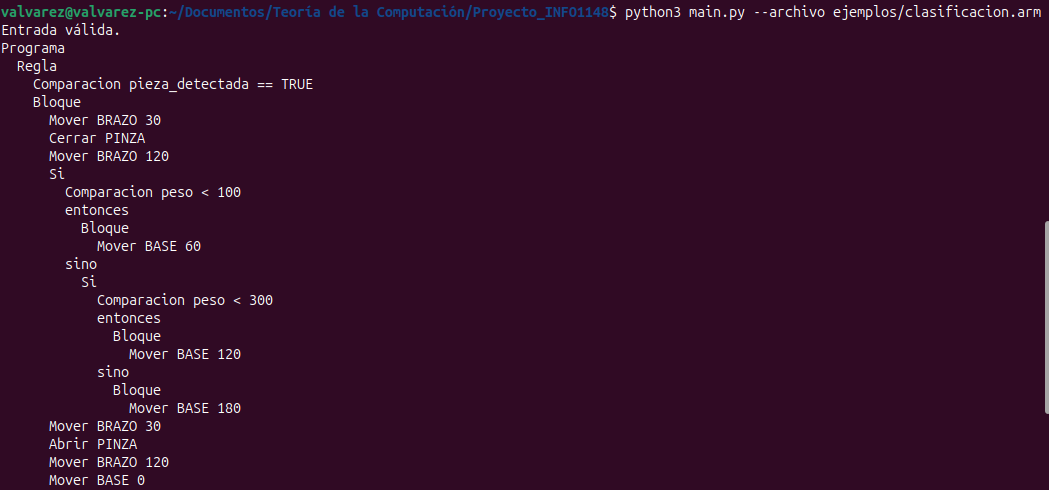
\includegraphics[
        width=\linewidth,
        height=0.70\textheight,
        keepaspectratio
    ]{figuras/clasificacion.png}
    \caption{Análisis del programa de clasificación: entrada
    aceptada y AST con decisión \tm{IF}--\tm{ELSE IF}--\tm{ELSE}
    y acciones del brazo del ciclo completo.}
    \label{fig:ejecucion_valida}
\end{figure}

\begin{figure}[H]
    \centering
    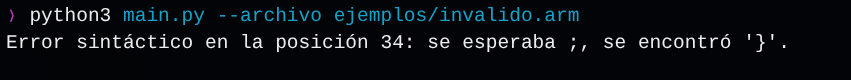
\includegraphics[width=\linewidth]{figuras/invalido.png}
    \caption{Rechazo de una entrada inválida: el analizador
    identifica la ausencia de punto y coma e informa la
    posición y el símbolo encontrado.}
    \label{fig:ejecucion_invalida}
\end{figure}

\begin{figure}[H]
    \centering
    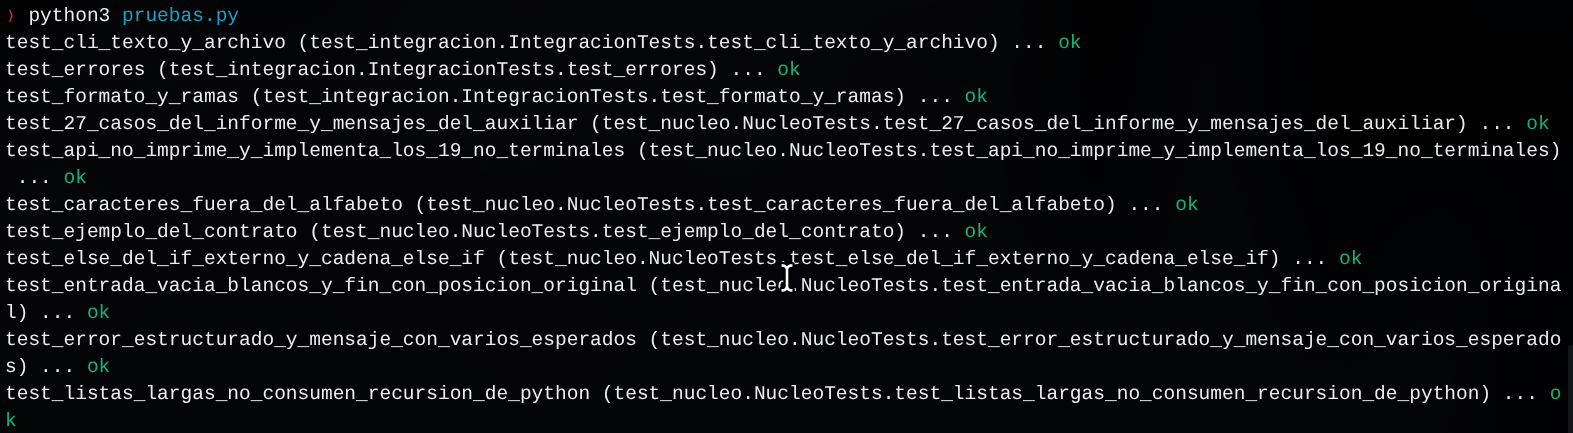
\includegraphics[width=\linewidth]{figuras/pruebas1.png}
    \caption{Primera parte de las pruebas automatizadas:
    comprobaciones de la interfaz, los 27 casos del informe,
    el análisis léxico y la estructura del AST.}
    \label{fig:pruebas_inicio}
\end{figure}

\begin{figure}[H]
    \centering
    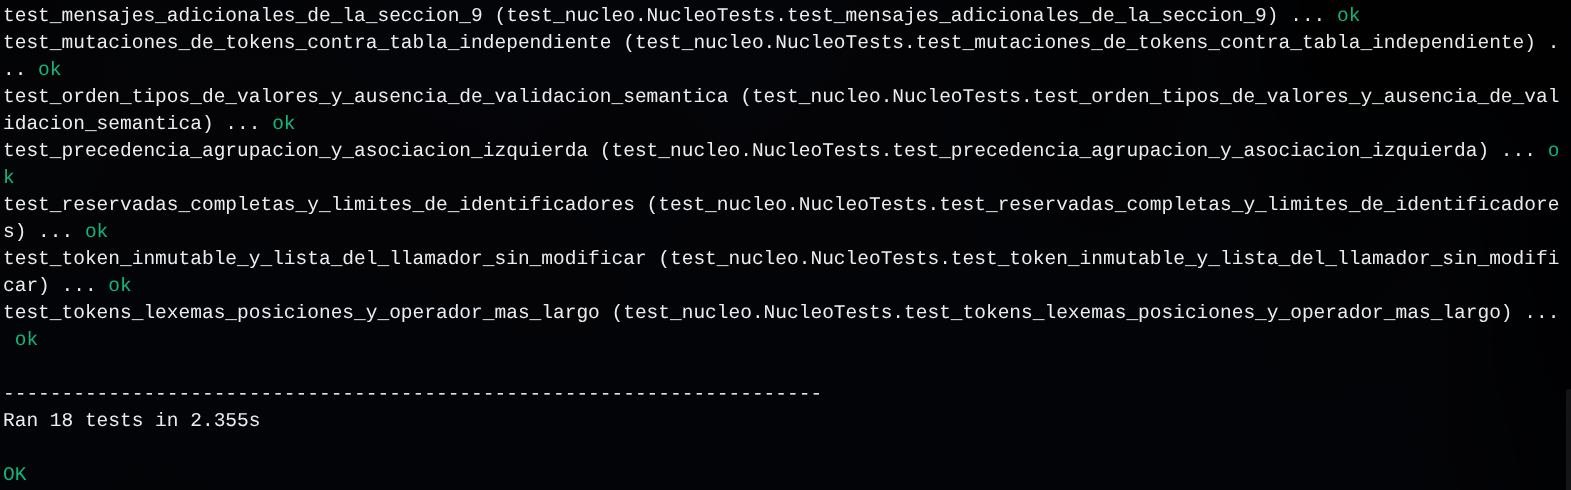
\includegraphics[width=\linewidth]{figuras/pruebas2.png}
    \caption{Continuación y resultado de las pruebas:
    las 18 pruebas automatizadas finalizan correctamente
    con el resultado \texttt{OK}.}
    \label{fig:pruebas_resultado}
\end{figure}


\section*{Anexo C. Definición formal completa de la gramática}
\hypertarget{anexoC}{}

\[
G = (V,\ \Sigma,\ P,\ S), \qquad S = \nt{programa}
\]

\textbf{Conjuntos}
\begin{itemize}[nosep]
\item $V = $ \ensuremath{\{}\nt{programa}, \nt{reglas}, \nt{regla}, \nt{bloque}, \nt{sentencias}, \nt{sentencia}, \nt{accion}, \nt{articulacion}, \nt{si}, \nt{sino}, \nt{sino\_cuerpo}, \nt{condicion}, \nt{condicion\_r}, \nt{conjuncion}, \nt{conjuncion\_r}, \nt{negacion}, \nt{primario}, \nt{comparacion}, \nt{valor}\ensuremath{\}}\ \ (19 no terminales).
\item $\Sigma = $ \ensuremath{\{}\tm{WHEN}, \tm{THEN}, \tm{IF}, \tm{ELSE}, \tm{MOVER}, \tm{ABRIR}, \tm{CERRAR}, \tm{BASE}, \tm{BRAZO}, \tm{PINZA}, \tm{AND}, \tm{OR}, \tm{NOT}, \tm{TRUE}, \tm{FALSE}, \tm{ID}, \tm{NUM}, \tm{OP\_REL}, \tm{;}, \tm{(}, \tm{)}, \tm{\{}, \tm{\}}\ensuremath{\}}\ \ (23 terminales).
\item $S = $ \nt{programa}.
\item $P = $ las 33 producciones de la lista numerada.\end{itemize}
\textbf{Producciones agrupadas por no terminal}
\begin{center}\small\begin{tabular}{@{}rl@{}}
\nt{programa} & $\rightarrow$ \nt{regla}\ \nt{reglas} \quad{\scriptsize(1)} \\
\nt{reglas} & $\rightarrow$ \nt{regla}\ \nt{reglas} $\mid$ $\varepsilon$ \quad{\scriptsize(2,3)} \\
\nt{regla} & $\rightarrow$ \tm{WHEN}\ \nt{condicion}\ \tm{THEN}\ \nt{bloque} \quad{\scriptsize(4)} \\
\nt{bloque} & $\rightarrow$ \tm{\{}\ \nt{sentencias}\ \tm{\}} \quad{\scriptsize(5)} \\
\nt{sentencias} & $\rightarrow$ \nt{sentencia}\ \nt{sentencias} $\mid$ $\varepsilon$ \quad{\scriptsize(6,7)} \\
\nt{sentencia} & $\rightarrow$ \nt{accion}\ \tm{;} $\mid$ \nt{si} \quad{\scriptsize(8,9)} \\
\nt{accion} & $\rightarrow$ \tm{MOVER}\ \nt{articulacion}\ \tm{NUM} $\mid$ \tm{ABRIR}\ \tm{PINZA} $\mid$ \tm{CERRAR}\ \tm{PINZA} \quad{\scriptsize(10,11,12)} \\
\nt{articulacion} & $\rightarrow$ \tm{BASE} $\mid$ \tm{BRAZO} \quad{\scriptsize(13,14)} \\
\nt{si} & $\rightarrow$ \tm{IF}\ \nt{condicion}\ \nt{bloque}\ \nt{sino} \quad{\scriptsize(15)} \\
\nt{sino} & $\rightarrow$ \tm{ELSE}\ \nt{sino\_cuerpo} $\mid$ $\varepsilon$ \quad{\scriptsize(16,17)} \\
\nt{sino\_cuerpo} & $\rightarrow$ \nt{si} $\mid$ \nt{bloque} \quad{\scriptsize(18,19)} \\
\nt{condicion} & $\rightarrow$ \nt{conjuncion}\ \nt{condicion\_r} \quad{\scriptsize(20)} \\
\nt{condicion\_r} & $\rightarrow$ \tm{OR}\ \nt{conjuncion}\ \nt{condicion\_r} $\mid$ $\varepsilon$ \quad{\scriptsize(21,22)} \\
\nt{conjuncion} & $\rightarrow$ \nt{negacion}\ \nt{conjuncion\_r} \quad{\scriptsize(23)} \\
\nt{conjuncion\_r} & $\rightarrow$ \tm{AND}\ \nt{negacion}\ \nt{conjuncion\_r} $\mid$ $\varepsilon$ \quad{\scriptsize(24,25)} \\
\nt{negacion} & $\rightarrow$ \tm{NOT}\ \nt{negacion} $\mid$ \nt{primario} \quad{\scriptsize(26,27)} \\
\nt{primario} & $\rightarrow$ \tm{(}\ \nt{condicion}\ \tm{)} $\mid$ \nt{comparacion} \quad{\scriptsize(28,29)} \\
\nt{comparacion} & $\rightarrow$ \tm{ID}\ \tm{OP\_REL}\ \nt{valor} \quad{\scriptsize(30)} \\
\nt{valor} & $\rightarrow$ \tm{NUM} $\mid$ \tm{TRUE} $\mid$ \tm{FALSE} \quad{\scriptsize(31,32,33)} \\
\end{tabular}\end{center}

$P$ es el conjunto de las 33 producciones de la sección~\ref{sec:gramatica_completa}. Los símbolos \tm{ID}, \tm{NUM} y
\tm{OP\_REL} son terminales que representan familias de cadenas, definidas formalmente en la sección~\ref{sec:alfabeto}.

\section*{Anexo D. Declaración de uso de inteligencia artificial}
\hypertarget{anexoD}{}

De acuerdo con las reglas del curso para proyectos, declaramos el uso de
herramientas de IA generativa en este trabajo:

\begin{itemize}[nosep]
\item \textbf{Claude} (Anthropic, Sonnet 5.5, octubre de 2026): apoyo en la
generación de ideas, y en la redacción, estructuración y revisión del informe.
\item \textbf{Codex} (OpenAI, GPT-6.1 Sol, octubre de 2026): apoyo en la creación del
código del analizador (léxico, parser, AST y pruebas).
\end{itemize}

\textbf{Autoría y diseño.} La elección del dominio (brazo robótico
clasificador), el diseño del lenguaje ARMLANG, la gramática, la extensión
creativa y las decisiones de diseño son de los integrantes del grupo. Las
herramientas de IA se utilizaron de forma guiada: les indicamos qué necesitábamos
en cada etapa y las dirigimos, mediante instrucciones y correcciones sucesivas,
hasta llegar al resultado que deseábamos. También las usamos para contrastar
ideas y explorar alternativas, y las decisiones finales las tomamos nosotros.

\textbf{Redacción del informe.} Claude se utilizó para redactar y estructurar el
texto a partir de nuestras indicaciones y del diseño ya definido por el grupo.
Cada sección fue revisada y algunas fueron ajustadas por nosotros cuando fue necesario.

\textbf{Código.} Codex se utilizó para crear el código a partir del diseño
del lenguaje y de la gramática. En todo momento analizamos y validamos lo que el
código hacía: comprobamos su correspondencia con la gramática y con las tablas
FIRST, FOLLOW y LL(1), ejecutamos los casos de prueba del informe y corregimos
lo necesario hasta obtener el comportamiento esperado.

\textbf{Referencias.} 

Anthropic. (2026). \emph{Claude} (Sonnet 5.5) [Modelo de lenguaje].
\url{https://claude.ai}.

OpenAI. (2026). \emph{Codex} (GPT-6.1 Sol) [Modelo de lenguaje].
\url{https://openai.com}.
\end{document}